\documentclass[10pt, a4paper]{article}
\usepackage[utf8]{inputenc}
\usepackage{url}
\usepackage{adjustbox}                % Balances the columns of the last page
\usepackage{amsmath}
\usepackage{amssymb}
\usepackage{amstext}
\usepackage[title]{appendix}
\usepackage{balance}                % Balances the columns of the last page
\usepackage{booktabs}
\usepackage{caption}
\usepackage{color}
\usepackage{enumerate}
\usepackage{fancyhdr}
    \usepackage[T1]{fontenc}
\usepackage{graphicx}
\usepackage[
  left=2cm,top=2.0cm,bottom=2.0cm,right=2cm,
  headheight=17pt, % as per the warning by fancyhdr
  includehead,includefoot,
  heightrounded, % to avoid spurious underfull messages
]{geometry}
\usepackage[colorlinks,linkcolor=blue]{hyperref}
\usepackage[utf8]{inputenc}
\usepackage{lipsum}
\usepackage{listings}
\usepackage{multicol}
\usepackage{multirow}
\usepackage[
    protrusion=true,
    activate={true,nocompatibility},
    final,
    tracking=true,
    kerning=true,
    spacing=true,
    factor=1100
]{microtype}
\usepackage{paralist}
\usepackage{pdfpages}
\usepackage{ragged2e}
\usepackage{rotating}
\usepackage{setspace}
\usepackage{subcaption}
\usepackage{tabularx}
\usepackage{tgbonum}
\usepackage{threeparttable}
\usepackage{times}
\usepackage{titlesec}
\usepackage{titling}
\usepackage[nottoc,numbib]{tocbibind}
\usepackage{tocloft}
\usepackage[colorinlistoftodos,prependcaption,textsize=normal]{todonotes}
\usepackage{xcolor}
\usepackage{xspace}
\usepackage{wrapfig}

% Must be loaded after hyperref
\usepackage[capitalise]{cleveref}  % Clever references to stuff.

\definecolor{codegreen}{rgb}{0,0.6,0}
\definecolor{codegray}{rgb}{0.5,0.5,0.5}
\definecolor{codepurple}{rgb}{0.58,0,0.82}
\definecolor{backcolour}{rgb}{0.95,0.95,0.92}

\lstdefinestyle{mystyle}{
    backgroundcolor=\color{backcolour},   
    commentstyle=\color{codegreen},
    keywordstyle=\color{magenta},
    numberstyle=\tiny\color{codegray},
    stringstyle=\color{codepurple},
    basicstyle=\ttfamily\footnotesize,
    breakatwhitespace=false,         
    breaklines=true,                 
    captionpos=b,                    
    keepspaces=true,                 
    numbers=left,                    
    numbersep=5pt,                  
    showspaces=false,                
    showstringspaces=false,
    showtabs=false,                  
    tabsize=2,
    mathescape
}

\lstset{style=mystyle}

\SetTracking{encoding={*}, shape=sc}{40}
\renewcommand{\familydefault}{\sfdefault}
\newcommand{\textFunc}[1]{\texttt{\textit{#1}}}
\newcommand{\code}[1]{\texttt{#1}}

\newcolumntype{C}[1]{>{\Centering}m{#1}}
\renewcommand\tabularxcolumn[1]{C{#1}}

\newcounter{rowcntr}[]
\renewcommand{\therowcntr}{\thesection.\arabic{rowcntr}}
% A new columntype to apply automatic stepping
\newcolumntype{N}{>{\refstepcounter{rowcntr}\therowcntr}c}
% Reset the rowcntr counter at each new tabular
\AtBeginEnvironment{tabular}{\setcounter{rowcntr}{0}}

\newcommand{\thesistitle}[0]{Model-Based Engineering for Quadcopter Control Software}
\newcommand{\authorname}[0]{Vrushank Agrawal}
\newcommand{\supervisor}[0]{Dr. Timothy Bourke}
\newcommand{\supervisorinstitution}[0]{INRIA / ENS / \'Ecole Polytechnique}

% Paragraph spacing
\setlength{\parskip}{1pt}%
\setlength{\parindent}{15pt}%

% set toc spacing
\renewcommand\cftchapafterpnum{\vskip1pt}
\renewcommand\cftsecafterpnum{\vskip1.5pt}

%  Start Document
\begin{document}
% \addtocontents{toc}{\protect\setcounter{tocdepth}{2}}
\pagenumbering{gobble}
\clearpage
\setcounter{figure}{0}

\begin{titlepage}
\begin{center}

    \begin{figure}
        \centering
        \begin{subfigure}[b]{0.35\textwidth}
            \centering
            
\includegraphics[width=\textwidth]{cool_logo.jpg}
            \label{figure:Polytechnique}
        \end{subfigure}
        \begin{subfigure}[b]{0.35\textwidth}
            \centering
            
\includegraphics[width=\textwidth]{logo-inria.png}
            \label{figure:Polytechnique}
        \end{subfigure}
        \label{figure:Cool Logos}
    \end{figure}

    \vspace*{2em}
    
    {\Large
        \textbf{\'Ecole Polytechnique}
        
        \vspace*{1em}
        \textit{BACHELOR THESIS IN COMPUTER SCIENCE}
        
        \vspace*{3em}
        {\huge \setstretch{1.3} \textbf{\thesistitle} \par}
    
        \vspace*{3em}
        
        \textit{Author:}\\
        \vspace*{0.5em}
        \authorname{}, \'Ecole Polytechnique
        
        \vspace*{0.5em}
        
        \textit{Advisor:}\\
        \vspace*{0.5em}
        \supervisor{}, \supervisorinstitution{}
        
        \vspace*{0.5em}
        
        \textit{Co-advisor:}\\
        \vspace*{0.5em}
        Basile Pesin, INRIA / ENS
    }
    
    \vspace*{15em}
    \textit{Academic year 2022/2023}

\end{center}
\end{titlepage}

\newpage
    \begin{center}
        {\huge \textbf{Abstract}}
    \end{center}
    \vspace*{5em}
    {\large \setstretch{1.3} The low-level software used to control Unmanned Aerial Vehicles (UAVs), like quadcopters and drones, is usually written in languages like C and C++. Model-Based Engineering is an alternative approach to writing programs where control algorithms are specified as high-level block diagrams from which code is automatically generated using tools like Simulink or Scade Suite. Block diagrams allow engineers to focus on describing and composing reactive behaviours of the systems which are hard to do directly from low-level languages. This thesis aims to study how much of a typical UAV controller can be adapted in a synchronous dataflow language. We will focus on the Crazyflie quadcopter, which has been developed for use in education and research and use the open-source Heptagon compiler to generate the C code that will be integrated into the Crazyflie firmware.
    \par}
    \vfill

\newpage
    \pagestyle{fancy}
    %\renewcommand{\headrulewidth}{0pt} % Remove line at top
    %\renewcommand{\headrulewidth}{0.4pt}% Default \headrulewidth is 0.4pt
    \lhead{\authorname}
    %\chead{\acronym}
    \rhead{\thesistitle}

\newpage
\tableofcontents

\clearpage
\pagenumbering{arabic}

\section{Introduction}
    In recent years, the demand for aircraft, specifically Unmanned Aerial Vehicles (UAV), with greater manoeuvrability and hovering ability has led to a significant rise in quadcopter research. A quadcopter (a type of drone) is a four-propeller helicopter, usually arranged in a square, with four independent rotors. The four-rotor design allows quadcopters to be relatively simple in design yet highly reliable and manoeuvrable, allowing them to be programmed for remote piloting by a ground control operator. Active research in the area continues to increase the abilities of quadcopters making them highly desirable for various civil and military applications such as environment exploration, land surveys, photography, remote strike execution, etc. With further research, quadcopters could be capable of advanced autonomous missions like agricultural monitoring and infrastructure inspection among other applications that are currently not possible with other vehicles \cite{article:quadcopter-intro}. One of the key challenges in this area of research, though, is the complexity of their software design which is usually written in low-level languages like C/C++.

    \subsection{Motivation}
    UAVs are safety-critical embedded systems that continuously interact in real time with their physical environment. This makes their behaviour very different from a compiler where data is available in the beginning or an interactive website where the operating system partly determines the interaction speed \cite{article:lustre-paper}. As such, UAVs need to be reactive in nature and thus use real-time operating systems that can dynamically make logical decisions as the input conditions change. Real-time operating systems use parallelism while adhering to time constraints and are hence written in low-level languages like C/C++ which allow precise control over system resources. However, low-level languages make these systems complex in nature which challenges engineers to define a clear mathematical model to reason about the system's behaviour during development, operation, and maintenance. Overall, system specifications generated from low-level languages are hard to validate which is a necessary industrial process because even a minor glitch in a commercial flight controller can be catastrophic.

    Model-Based Engineering is an alternative approach to designing UAVs by using synchronous dataflow languages. With this approach, the algorithms and states of embedded systems are specified as high-level block diagrams while tools like Simulink and Scade Suite \cite{web:Scade-Suite} are used to automatically transform the code into a low-level language such as C. This methodology allows programmers to visualize the software as reacting instantaneously to external events at a known time. It also enables programmers to think of their software in terms of the flow of data where the software reacts deterministically according to a set of mathematical equations defined in the blocks. Synchronous dataflow languages also provide a mathematically simpler model with a high-level abstraction that is easier to understand and formally verify compared to software written in low-level languages. The high-level code is also reusable and easier to maintain resulting in improved software quality while reducing the software development time.

    \begin{figure}[hbt!]
        \centering
        \begin{subfigure}[b]{0.28\linewidth}
        \rotatebox{90}{
                \centering
                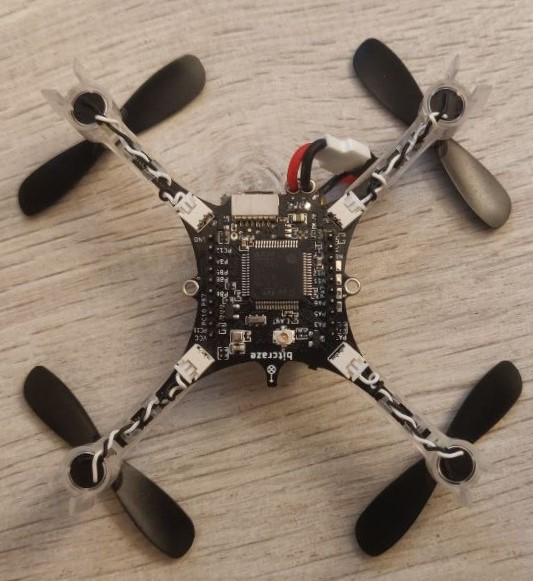
\includegraphics[width=\linewidth]{back.jpg}
            }
            \caption{Bottom View.}
            \label{figure:bottom}
        \end{subfigure}
        \hfill
        \begin{subfigure}[b]{0.35\textwidth}
            \centering
            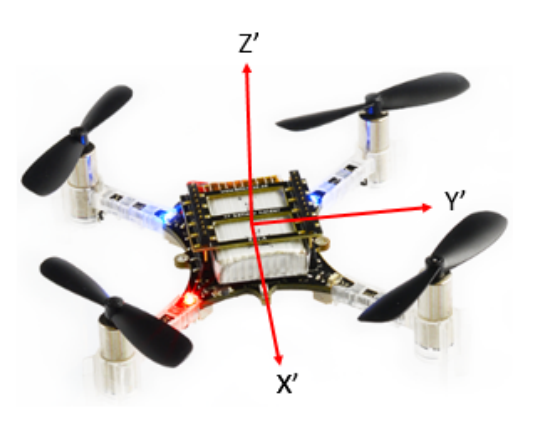
\includegraphics[width=\textwidth]{axes2.png}
            \caption{Axes}
            \label{figure:axes}
        \end{subfigure}
        \hfill
        \begin{subfigure}[b]{0.31\textwidth}
            \rotatebox{180}{%
                \centering
                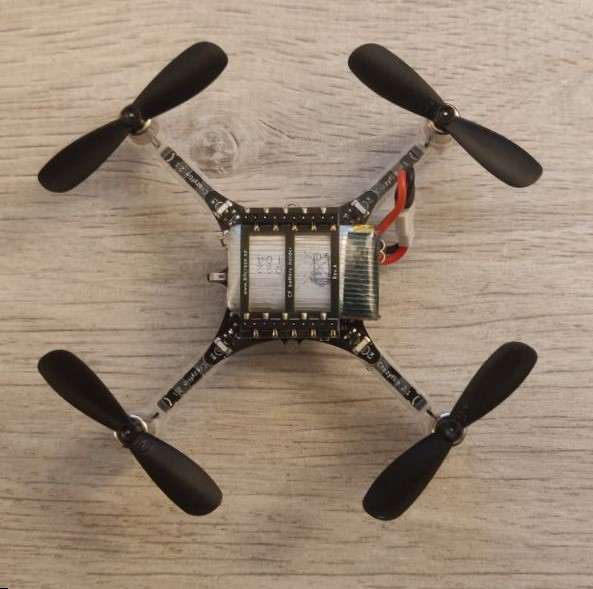
\includegraphics[width=\textwidth]{front.jpg}    
                }
            \caption{Top View}
            \label{figure:axes}
        \end{subfigure}
        \caption{Crazyflie 2.1 quadcopter}
        \label{figure:Crazyflie}
    \end{figure}  

    \subsection{Objective}
    The objective of this thesis is to implement portions of a quadcopter's feedback control loop in Heptagon, a synchronous dataflow language and an extension of Lustre \cite{article:lustre-paper}. The thesis will explore the question of how much of the low-level code of a typical UAV can be written in a synchronous dataflow language. The study will focus on the Bitcraze Crazyflie 2.1 quadcopter (figure \ref{figure:Crazyflie}) which has specifically been developed for testing and research purposes. The Crazyflie uses an ARM Cortex-M4, a $1$Mb flash, and the Bosch electronics' BMI$088$ 3 axis accelerometer/gyroscope and the BMP$388$ high precision pressure sensor \cite{web:crazyflie-2.1}. The Crazyflie firmware (source code for Crazyflie) will be implemented as Heptagon nodes (see section \ref{section:Heptagon}) which will be converted into C code using the open-source Heptagon compiler \cite{software:heptagon-compiler}. The Heptagon-generated C code will be used to replace the original source code in the Crazyflie firmware to evaluate the correctness of the Heptagon version. Initially, the controller (section \ref{section:controller}) and estimator (section \ref{section:estimator}) will be converted to Heptagon nodes as they are relatively simple to implement. Subsequently, FreeRTOS tasks (section \ref{section:freeRTOS_tasks}) will be converted to Heptagon nodes and integrated into the Crazyflie firmware. By implementing a quadcopter's low-level code in Heptagon, the thesis aims to demonstrate the feasibility of using a synchronous dataflow language to develop software for UAVs.

    \subsection{Context}
    This thesis builds on the findings of the report "Software Engineering for Quadcopter Control" \cite{report:cse303-report} which was a result of the course CSE303---Computer Science Project.  The objective of the project was to understand the feedback control loop of the Crazyflie 2.1 and how it interacts with the overall process of the quadcopter by performing simple experiments. This was done to analyze the feasibility of converting the UAV's low-level C code into a high-level synchronous dataflow language like Lustre. A conclusion of the report asserted that the design of Crazyflie's control loop was well-understood and feasible to be implemented in Lustre. Figure \ref{figure:previous-block-diagram} in appendix \ref{appendix:previous-block-diagram} is the block-diagram representation of Crazyflie's feedback control loop implemented on its firmware version $2022.09$ \cite{software:Crazyflie-github-previous-version}. The block-diagram was a result of the report and provides the starting point for this thesis (section \ref{section:contributions}).

\section{Background}
    This section provides a comprehensive understanding of the fundamental concepts necessary to understand the contributions discussed in the thesis. It provides a background on Heptagon which is a dataflow synchronous language and explores the physics behind the movement of the quadcopter. The section also covers concepts like quaternions, schedulers, feedback control loops, state estimation and control algorithms that are all used in a typical UAV.

    \subsection{Heptagon - synchronous dataflow language}
    \label{section:Heptagon}
    Heptagon is a dataflow synchronous language whose syntax and semantics are inspired by Lustre \cite{software:heptagon-compiler}. Lustre was originally designed for programming reactive systems such as  automatic control and monitoring systems. Its dataflow aspect makes it very close to the usual description tools used in these domains such as block-diagrams, and its synchronous interpretation makes it well suited for handling temporal programs \cite{article:lustre-paper}. Hence, using Heptagon to translate Crazyflie's code into a synchronous dataflow language allows us to exploit the dataflow nature of Lustre as well as the modern features provided by Heptagon like control structures such as switch and automata.

    All variables and expressions in Heptagon denote a flow of data, like a sequence of elements flowing in time. These variables and expressions can be coupled together to create a \textFunc{node} ($f$) also called a subprogram. The node has inputs ($x_1, \dots x_n$), outputs ($y_1, \dots y_n$), and local variables ($z_1, \dots z_n$) where each variable has a specific data type let's say ($t_1, \dots t_n$), ($t_1^{'}, \dots t_n^{'}$), and ($t_1^{''}, \dots t_n^{''}$) respectively. These inputs, outputs, and local variables are acted upon by declarations ($D$) (shown in listing \ref{listing:Heptagon_node}) that can apply the usual operators (e.g. Boolean and arithmetic) pointwise on the sequences of the variables (shown in table \ref{table:Heptagon_node}). Each variable in a node can be assigned one and only one expression. Finally, a Heptagon program is structured as a sequence of \textFunc{nodes} \cite{report:heptagon_manual}.
    \clearpage

    \begin{lstlisting}[caption={A node in Heptagon}, label={listing:Heptagon_node}, language=C]
node $f(x_1:t_1; \quad\hdots;\quad x_n:t_n$) returns ($y_1:t_1^{'}; \quad\hdots;\quad y_n:t_n^{'}$);
var $z_1:t_1^{''}; \quad\hdots;\quad z_n:t_n^{''}$;
let
  $D$
tel     \end{lstlisting}

    \begin{minipage}{\linewidth}
    \centering
    \captionof{table}{Pointwise addition on Heptagon variables.}
    \label{table:Heptagon_node} 
    \begin{tabular}{ C{0.95in} | C{.38in} | *5{C{.38in}}}\toprule[1.5pt]
        \toprule[1.5pt]
        \bf Time    &        & $1$ & $2$ & $3$ & $4$ & \dots \\
        \midrule
        \bf Variable & \bf x & $x_1$ & $x_2$ & $x_3$ & $x_4$ & \dots \\
        \midrule
        \bf Variable & \bf y & $y_1$ & $y_2$ & $y_3$ & $y_4$ & \dots \\
        \midrule
        \bf Expression & \bf x+y & $x_1 + y_1$ & $x_2 + y_2$ & $x_3 + y_3$ & $x_4 + y_4$ & \dots \\
        \bottomrule[1.25pt]
    \end{tabular}\par
    \end{minipage}

    \subsubsection{Syntactic extensions}
    \label{section:syntactic-extensions}
    Heptagon incorporates several modern syntax features in Lustre. Within these, the three main Heptagon-specific syntactic features used in this thesis are explained in the following.
    \\ \\
    \textbf{Follow By (fby)}
    \\ \\
    Follow by (fby) is a type of delay in Heptagon. Listing \ref{listing:Heptagon_fby} gives an example of a node that uses a follow by. The node \textFunc{everyn()} accepts one input stream $n$ which contains integer values and outputs another stream $v$ of booleans. It also contains an internal stream of integers $x$ and the equation in line \ref{line:flow-of-x} defines this stream. This equation can be literally translated to "x is zero followed by $(x+1)\%n$" which means that $x$ is a stream that starts with zero and followed by an increasing sequence of natural numbers which is calculated "\textFunc{modulo n}", and hence, reset to zero every $n$ iterations. Line \ref{line:flow-of-v} defines the stream of values for $v$ where the current value of element is set to \textbf{\textit{true}} if $x$ is zero otherwise \textbf{\textit{false}}. These streams of values can be visualized as a flow in table \ref{table:Heptagon_fby} where $n=3$.

    \begin{lstlisting}[caption={Sample Heptagon code with follow bys}, label={listing:Heptagon_fby}, language=C]
node everyn(n : int) returns (v : bool);
var x : int;
let
  x = 0 fby ((x + 1) % n);  $\label{line:flow-of-x}$
  v = (x = 0);              $\label{line:flow-of-v}$
tel     \end{lstlisting}

    \begin{minipage}{\linewidth}
    \centering
    \captionof{table}{Dataflow for \textFunc{everyn(3)} in listing \ref{listing:Heptagon_fby}.}
    \label{table:Heptagon_fby} 
    \begin{tabular}{ C{0.95in} *9{C{.38in}}}\toprule[1.5pt]
        \toprule[1.5pt]
        \bf Clock & 1 & 2 & 3 & 4 & 5 & 6 & 7 & 8 & 9\\
        \midrule
        \bf x & 0 & 1 & 2 & 0 & 1 & 2 & 0 & 1 & 2\\
        \midrule
        \bf v & true & false & false & true & false & false & true & false & false\\
        \bottomrule[1.25pt]
    \end{tabular}\par
    \end{minipage}
    \bigskip
    \\ \\
    \textbf{Automata}
    \\ \\
    Automata or a state machine is a type of control structure in Heptagon. It is a set of states (each with its own declaration) as well as the transitions between these states triggered by Boolean expressions \cite{report:heptagon_manual}. The node \textFunc{led\_on\_every\_n()} in listing \ref{listing:Heptagon_automaton} is an example of automata (line \ref{line:automata}) composed of two states---ON (line \ref{line:state-ON}) and OFF (line \ref{line:state-OFF})---that return \textFunc{true} and \textFunc{false} respectively. When the node is running, the switching of states inside the automata happens instantaneously based on the value of the \textFunc{timer} stream which is evaluated for a boolean expression. Based on the value of the evaluated boolean expression, the switching happens instantaneously because of the \textFunc{unless} keyword (lines \ref{line:unless-1} and \ref{line:unless-2}) which effects a strong transition \cite{report:heptagon_manual}. The code for the strong transition in listing \ref{listing:Heptagon_automaton} is better visualized in table \ref{table:Heptagon_automaton} where $n=2$.

    \begin{lstlisting}[caption={Sample Heptagon code with automaton control structure}, label={listing:Heptagon_automaton}, language=C]
node led_on_every_n(n : int) returns(led_state : bool);
var timer : int;
let
    timer = (0 fby (timer+1)) % n;
    automaton                               $\label{line:automata}$
        state ON                               $\label{line:state-ON}$
            do led_state = true
            unless (timer > 0) then OFF      $\label{line:unless-1}$
        state OFF                               $\label{line:state-OFF}$
            do led_state = false
            unless (timer = 0) then ON       $\label{line:unless-2}$
    end;
tel     \end{lstlisting}

    \begin{minipage}{\linewidth}
    \centering
    \captionof{table}{Dataflow for \textFunc{led\_on\_every\_n(2)} in listing \ref{listing:Heptagon_automaton}.} 
    \label{table:Heptagon_automaton} 
    \begin{tabular}{ C{0.95in} *9{C{.38in}}}\toprule[1.5pt]
        \toprule[1.5pt]
        \bf Clock & 1 & 2 & 3 & 4 & 5 & 6 & 7 & 8 & 9\\
        \midrule
        \bf \textFunc{last} timer & 0 & 1 & 0 & 1 & 0 & 1 & 0 & 1 & 0\\
        \midrule
        \bf led\_state & true & false & true & false & true & false & true & false & true\\
        \bottomrule[1.25pt]
    \end{tabular}\par
    \end{minipage}
    \bigskip
    \\ \\
    \textbf{Switch}
    \\ \\
    Switch is another type of control structure in Heptagon where the set of equations that apply at any instant are determined by a conditional expression. Listing \ref{listing:Heptagon_switch} gives an example where the switch control structure is used to switch the equations that are evaluated at that instant based on the conditional expression. Line \ref{line:action-mode} defines a type variable that is used in the conditional expression evaluated by the switch control structure in lines \ref{line:switch-start}-\ref{line:switch-end}. The \code{last} keyword in line \ref{line:switch-last-keyword} simply instructs Heptagon to take the last value from the variable's stream of values. To use the \code{last} keyword, the variable must be initialized with a last value as done in line \ref{line:switch-last-def} where \textFunc{led\_state} of type \textFunc{bool} is initialized with \textFunc{false}. The dataflow for the node can be visualized in table \ref{table:Heptagon_switch}.

    \begin{lstlisting}[caption={Sample Heptagon code with switch control structure}, label={listing:Heptagon_switch}, language=C]
type action = Change | Previous                 $\label{line:action-mode}$

node ledseq_task(led_action: action) returns(last led_state : bool = false);   $\label{line:switch-last-def}$
let
    switch (led_action)                         $\label{line:switch-start}$
    | Change do led_state = led_on_every_n(2)
    | Previous do led_state = last led_state    $\label{line:switch-last-keyword}$
    end;                                        $\label{line:switch-end}$
tel     \end{lstlisting}

    \begin{minipage}{\linewidth}
    \centering
    \captionof{table}{Dataflow for \textFunc{ledseq\_task} in listing \ref{listing:Heptagon_switch}.} 
    \label{table:Heptagon_switch}
    \begin{tabular}{ C{0.95in} *8{C{.45in}}}\toprule[1.5pt]
        \toprule[1.5pt]
        \bf Clock & 1 & 2 & 3 & 4 & 5 & 6 & 7 & 8 \\
        \midrule
        \bf led\_action & Previous & Change & Change & Change & Previous & Previous & Previous & Change\\
        \midrule
        \bf led\_state & false & true & false & true & true & true & true & false\\
        \bottomrule[1.25pt]
    \end{tabular}\par
    \end{minipage}

    \subsubsection{External functions interface}
    Heptagon offers the possibility to import external functions that cannot be defined within Heptagon. These functions can be defined in a \code{.epi} file and they must respect Heptagon calling conventions as described in appendix A of the Heptagon/BZR manual \cite{report:heptagon_manual}. Listing \ref{listing:Heptagon-external} defines trigonometric functions that are imported from the C math library that can be used inside Heptagon. Interface files (\code{.epi}) can be compiled with the \code{heptc} command to generate a compiled interface with the extension \code{.epci} \cite{report:heptagon_manual}.

    \begin{lstlisting}[caption={External function definitions in .epi file}, label={listing:Heptagon-external}, language=C]
external val fun sin(x:float) returns (y:float)
external val fun cos(x:float) returns (y:float)
external val fun tan(x:float) returns (y:float)     \end{lstlisting}

    \subsection{Rotations of a quadcopter}

    \begin{figure}[hbt!]
        \centering
        \begin{subfigure}[b]{0.51\textwidth}
            \centering
            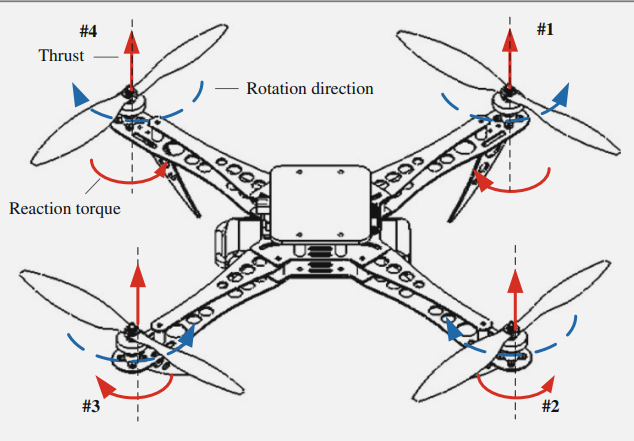
\includegraphics[width=\textwidth]{rotation.png}
            \caption{Propeller rotation}
            \label{figure:rotate}
        \end{subfigure}
        \hfill
        \begin{subfigure}[b]{0.41\textwidth}
            \centering
            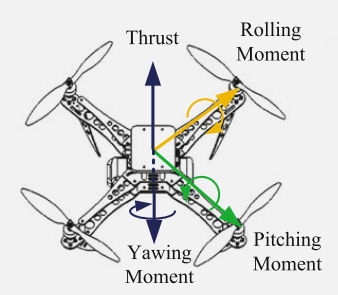
\includegraphics[width=\textwidth]{rot_dof.png}
            \caption{Rotational Degrees of Freedom}
            \label{figure:rot_DOF}        
        \end{subfigure}
        \caption{Quadcopter Rotation and Degrees of Freedom \cite{book:quan2017-movements}}
        \label{figure:DOF}
    \end{figure}

    A quadcopter uses 4 propellers divided into 2 sets of diagonal pairs which rotate clockwise and anti-clockwise respectively. A pair of propellers on the same side spin in the opposite direction, i.e. diagonal propellers spin in the same direction. This is done to nullify the torque generated as a reaction of the upward force generated when the propellers rotate with some angular speed as shown in figure \ref{figure:rotate}. A quadcopter has 6 degrees of freedom where 3 degrees are for transitional movement along the x, y, and z axes while 3 degrees are for rotational movement along the same axes termed roll, pitch, and yaw respectively as shown in figure \ref{figure:rot_DOF} \cite{article:pid-controller-IIJEM}. Roll, pitch, and yaw are together called \textFunc{attitude} of a UAV. Even with $6$ degrees of freedom, it is possible to control the movement of a quadcopter by using only four of them: thrust, roll, pitch, and yaw \cite{book:quan2017-movements} as explained below and illustrated in figure \ref{figure:Movements}.

    \begin{itemize}
        \item \code{Thrust}: It is the transitional movement along the z-axis or \textit{upward-and-downward movement} \cite{book:quan2017-movements}. It is controlled by changing the angular speed of the propellers by an equal amount as shown in figure \ref{figure:Thrust}. All motors change angular speed with the same amount and as a result, there is a net upward force on the quadcopter. So, if the quadcopter needs to rise, the angular speed of the propellers will be increased proportionally to increase the upward force acting on it.
    
        \item \code{Roll}: It is the rotational movement along the x-axis or \textit{leftward-and-rightward movement} \cite{book:quan2017-movements}. If the quadcopter wants to roll right, it would speed up motors on the left side ($\#3, \#4$) by some amount and slow down the two on the right ($\#1, \#2$) by the same amount as shown in figure \ref{figure:roll}. Doing this creates an increased net force on the left side which lifts it there to produce a right roll.

        \item \code{Pitch}: It is the rotational movement along the y-axis or \textit{forward-and-backward movement} \cite{book:quan2017-movements}. If the quadcopter wants to pitch forward, it speeds up the two motors at the back ($\#3, \#2$) and slows down the two at the front ($\#1, \#4$) as shown in figure \ref{figure:pitch}. Doing this increases the torque at the back end of the quadcopter and it rises up relative to the inertial frame generating a forward pitching movement.
                
\begin{figure}[hbt!]
    \centering
    \begin{subfigure}[b]{0.41\textwidth}
        \centering
        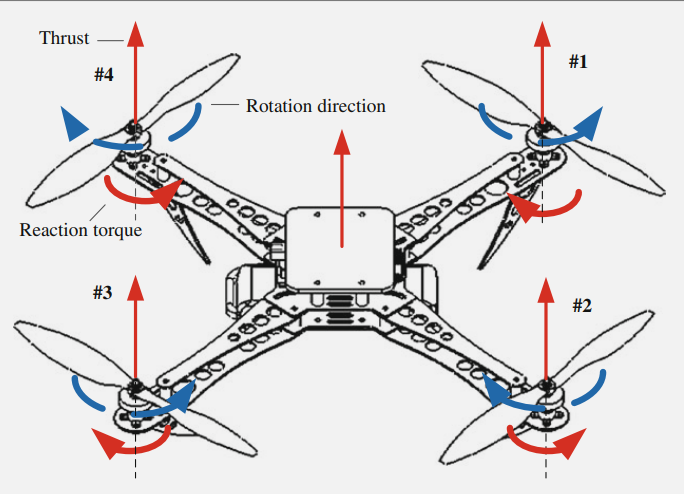
\includegraphics[width=\textwidth]{thrust.png}
        \caption{Upward Thrust}
        \label{figure:Thrust}
    \end{subfigure}
    \hfill
    \begin{subfigure}[b]{0.45\textwidth}
        \centering
        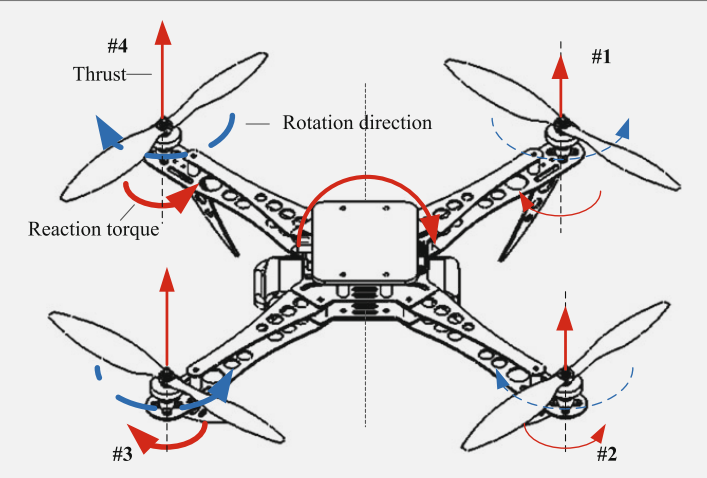
\includegraphics[width=\textwidth]{roll.png}
        \caption{Right Roll}
        \label{figure:roll}        
    \end{subfigure}
    \hfill
    \begin{subfigure}[b]{0.45\textwidth}
        \centering
        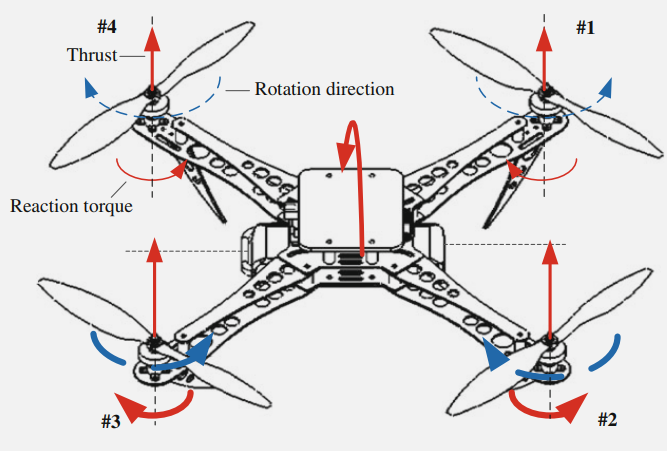
\includegraphics[width=\textwidth]{pitch.png}
        \caption{Forward Pitch}
        \label{figure:pitch}        
    \end{subfigure}
    \hfill
    \begin{subfigure}[b]{0.41\textwidth}
        \centering
        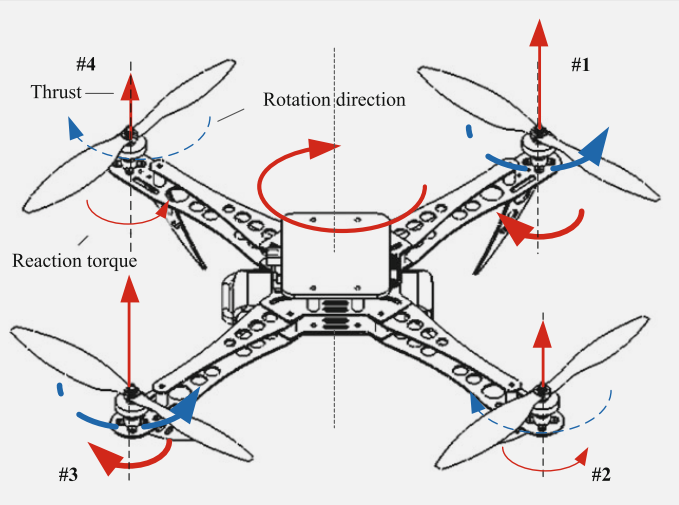
\includegraphics[width=\textwidth]{yaw.png}
        \caption{Clockwise Yaw}
        \label{figure:yaw}        
    \end{subfigure}
    \caption{Quadcopter movements as a result of the change in motor angular speeds \cite{book:quan2017-movements}.}
    \label{figure:Movements}
\end{figure}

        \item \code{Yaw}: It is the rotational movement along the z-axis or \textit{clockwise-and-anticlockwise movement}. This movement is realized by increasing and decreasing the angular speed of the diagonal propellers by the same amount. If the quadcopter wants to yaw clockwise, the angular speed of the propellers rotating clockwise ($\#4, \#2$) will be decreased while the angular speed of the propellers rotating anti-clockwise ($\#1, \#3$) will be increased by the same amount as shown in figure \ref{figure:yaw}. A net unequal reactionary torque would be generated in the clockwise direction relative to the copter's z-axis turning it clockwise.
    \end{itemize}

    \subsection{Quaternions}
    \label{section:quaternions}

    \begin{figure}[hbt!]
        \centering
        \begin{subfigure}[b]{0.35\textwidth}
            \centering
            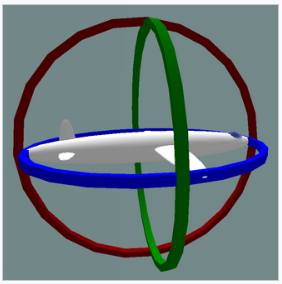
\includegraphics[width=\textwidth]{normal-gimbal.png}
            \caption{Non-aligned gimbals.}
            \label{figure:normal-gimbal}
        \end{subfigure}
        % \hfill
        \begin{subfigure}[b]{0.35\textwidth}
            \centering
            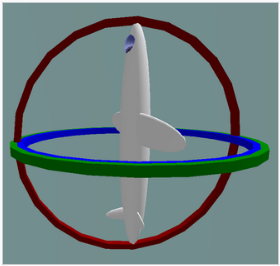
\includegraphics[width=\textwidth, angle=270]{gimbal-lock.png}
            \caption{Gimbal lock.}
            \label{figure:gimbal-lock}
        \end{subfigure}
        \hfill
        \caption{Gimbal system to represent $3D$ rotations \cite{image:gimbals}.}
        \label{figure:gimbals}
    \end{figure}

    Euler angles are a set of three angles that offer an intuitive method for representing three-dimensional rotations. In this system, three gimbals (rings suspended to rotate about an axis) are used to allow an object to rotate around one of the three X, Y, and Z axes (figure \ref{figure:normal-gimbal}). Though, due to this axis-angle representation, it is possible for two rings to align and lose one degree of freedom which is called the Gimbal lock (figure \ref{figure:gimbal-lock}). Gimbal locks make Euler angles extremely dangerous for applications in aviation as they can potentially reduce the degrees of freedom of a UAV from three to one when all gimbals get aligned. An alternate method to represent three-dimensional rotations is to use quaternions for the attitude representation of UAVs. Quaternions do not suffer from gimbal locks and are faster to compute since trigonometric computations are not needed \cite{article:quadrocopter_quaternions}.

    Quaternions are a mathematical concept first introduced by William Hamilton in 1843. They extend the complex numbers to four-dimensions. A quaternion $q \in \mathbb{R}^4$ is normally written as $\bf q \triangleq [w \quad \bf v]^T$ where $w \in \mathbb{R}$ is the scalar part and $\bf v = [x\quad y\quad z]^T \in \mathbb{R}^3$ is the vector part of the quaternion \cite{book:quan2017-quaternions}. Quaternions obey basic operation rules such as addition, subtraction, multiplication, norm, conjugate, inverse, and division and are widely used to represent three-dimensional rotations. Their relationship with three-dimensional rotations is neatly described in the following theorem (see \cite{book:quan2017-quaternions} for the proof):
    
    \noindent \textbf{Theorem}: Let $p$ be a point in three-dimensional space, represented in quaternion notation as $$p = [w \quad (x\quad y\quad z)]^T = [w \quad \bf v]^T$$ If $q$ is a non-zero quaternion, then the following statements hold:
    \begin{enumerate}
        \item The product $qpq^{-1}$ sends $p=[w\quad v]^T$ to $p'=[w\quad v']^T$ where $\lVert v\rVert = \lVert v'\rVert$.
        \item Any non-zero real multiple of $q$ gives the same action.
        \item If $\lVert q \rVert = 1$, then $q=[\cos \theta \quad \hat{v} \sin \theta]^T$ represents a rotation where $\lVert\hat{v}\rVert=1$. Now, $q$ acts to make a vector $v_t \in \mathbb{R}^3$ rotate around the unit axis $\hat{v}$ by $2\theta$ to achieve ${v_t}^{'} \in \mathbb{R}^3$.
    \end{enumerate}

    A direct result of the above theorem states that every $3D$ rotation corresponds to a unit quaternion \cite{book:quan2017-quaternions}. This property makes unit quaternions less prone to numerical errors once they are normalized. Furthermore, if there are two rotations $q_1, q_2 \in \mathbb{R}^4$ such that $q=q_2 q_1 \in \mathbb{R}^4$, then $q$ represents the rotation $q_1$ followed by $q_2$ because $q_2(q_1p{q_1}^{*}){q_2}^{*} = (q_2q_1)p({q_1}^{*}{q_2}^{*}) = qpq^{*}$ \cite{book:quan2017-quaternions}. Essentially, quaternions can easily represent interpolations between two rotations which is essential for UAV control systems. Overall, all the properties mentioned justify the use of quaternions for the attitude representation of UAVs.

    \subsection{FreeRTOS scheduler}
    FreeRTOS is an open-source real-time operating system designed for microcontrollers and also used in the Crazyflie. It has been developed in partnership with the world's leading chip companies over an 18-year period, and hence, has a large user community which has created a rich ecosystem of development tools. This community actively contributes to the development of new features to extend FreeRTOS functionality while providing crucial support for the platform. The FreeRTOS operating system supports many architectures and provides a reliable framework for multitasking, parallelism, and memory management. Furthermore, it is designed to operate in a resource-constrained environment \cite{web:freertos-kernel}. These features together make FreeRTOS an ideal pick for embedded systems like UAVs which have limited resources, require precise timing, and need safe inter-task communication capabilities.

    A scheduler, on the other hand, is a software routine in an operating system that regularly delegates computing resources to tasks. In FreeRTOS, the scheduling algorithm decides which task should be in the running state at a certain point in time. There can always be only one task in the running state per processor core at any given time.

    \subsubsection{Tasks}
    \label{section:freeRTOS_tasks}
    A Real-time operating system (RTOS) can be structured as a set of tasks run by a scheduler where each task executes within its own context with no operational authority on other tasks within the system. At any instant, only the scheduler decides which task executes on the micro-controller and any task itself has no knowledge of the scheduler activity. Furthermore, it is the responsibility of the scheduler to ensure that the processor context (register values, stack contents, etc) when a task is swapped in is the same as when the same task was swapped out. This is achieved by providing individual stacks for each task \cite{web:tasks-and-coroutines}.

    In FreeRTOS, tasks are implemented as C functions. Each task behaves like a small independent program which has a single entry point and will normally run forever with no exit. Consequently, these tasks never return from the function and hence if they are no longer needed they must be deleted. In FreeRTOS, tasks can be either in a Running state or one of the three Not Running states explained later in this section. In the Running state, the processor executes the running task's code while in the Not Running state, the status of the task is saved for possible future execution. The FreeRTOS scheduler is the only entity that can change the status of a task from Not Running to Running in which case it is said to 'switch in' the task \cite{book:freertos-guide-tasks}.

    The Not Running superstate has three sub-states: Blocked, Suspended and Ready states. A task waiting for a specific event to occur is said to be in the Blocked state. A task can enter a Blocked state due to temporal (time-related) or synchronization events. In a temporal event, the task must wait in the Blocked state for a specific time interval, for example, $10$ milliseconds. In case of a synchronization event, the task must wait in the Blocked state until another task or interrupt is executed, for example waiting for data to arrive on a queue. A task is said to be in the Suspended state it is not available to be called by the scheduler. A task may enter this state only if it is called by the \code{vTaskSuspend()} FreeRTOS API function. A task may leave the Suspended state only through a call by the \code{vTaskResume()} or \code{xTaskResumerFromISR()} FreeRTOS API functions \cite{book:freertos-guide-tasks}. Finally, a task is said to be in the Ready state if they are neither in the Blocked nor the Suspended states. These tasks are able to run but are waiting to be 'switched in' by the scheduler and enter the Running state. Figure \ref{figure:task-state-machine} shows the detailed state diagram for FreeRTOS tasks with the relevant API functions.

\begin{figure}[hbt!]
    \centering
    \begin{subfigure}[b]{0.41\textwidth}
        \centering
        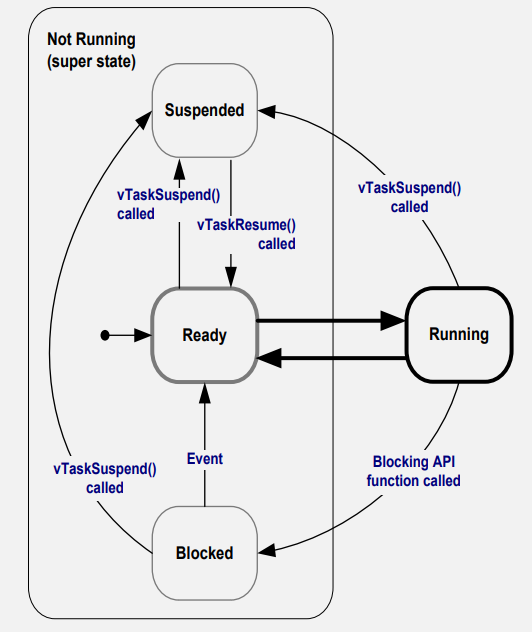
\includegraphics[width=\textwidth]{task-state-machine.png}
    \end{subfigure}
    \caption{FreeRTOS task state machine \cite{book:freertos-guide-tasks}.}
    \label{figure:task-state-machine}
\end{figure}

    \subsubsection{Preemptive scheduler}
    \label{section:preemptive-scheduler}
    The Crazyflie 2.1 uses the preemptive scheduler (see appendix \ref{software-reference:crazyflie-github-scheduler-type}) \cite{book:freertos-guide-preemptive} that decides which of the ready in-memory tasks to run after every clock interrupt. A preemptive scheduler has the capability of forcibly stopping tasks of lower priority if a process of a higher priority is ready to run. As an example, let us assume that an interrupt service routine (ISR) dynamically increases the priority of a task that is able to run. In this case, the scheduler will stop the lower-priority task currently running and start the higher-priority task even if the task is in the middle of a time slice. Here, the higher priority task is said to have "preempted" the lower priority task \cite{web:freertos-scheduling}. In the Crazyflie, a maximum priority of $5$ can be set (see appendix \ref{software-reference:crazyflie-github-maxTaskPriority}) where $5$ is the highest priority and $0$ is the lowest priority \cite{book:freertos-guide-tasks}.

    The priority-based scheduling aspect of the preemptive scheduler makes it non-deterministic in nature as it does not consider the execution time of the tasks. This introduces the possibility that a higher-priority task may repeatedly preempt a lower-priority task which will not get enough CPU resources due to lack of execution time (shown in figure \ref{figure:timeflow_reading2}) making the system unpredictable and the replication of reactive behaviours difficult.

    \subsubsection{Idle task}
    \label{section:idle-task}
    As explained in section \ref{section:freeRTOS_tasks}, a task can be parked in the Blocked state where it is not available to be run by the scheduler. In such a scenario, it is possible that no user-defined task is in the Running or the Ready state, but in FreeRTOS, there must always be at least one task that is in the Ready state to be 'switched in' the Running state if needed. As a workaround for this issue, the FreeRTOS scheduler automatically creates an idle task as soon as it is called by the \textFunc{vTaskStartScheduler()} API function. This task cannot be put in the Blocked or the Suspended state and is hence always available to be run. Furthermore, it has a priority of zero and can thus be preempted by a task of a higher priority. The idle task is responsible for cleaning up kernel resources after a task has been deleted, but other than that, it essentially runs an empty infinite loop \cite{book:freertos-guide-tasks}.

    \subsection{Feedback control}
    \label{section:feedback-control}
    The feedback control loop is an essential software mechanism in a UAV that allows the UAV to operate autonomously. It is responsible for measuring the current state of the UAV and using relevant control algorithms to moderate the input of the UAV's hardware. For the Crazyflie, this hardware input is the thrust provided individually to each of the four motors. A feedback control loop can be either open or closed. An open-loop control mechanism takes decisions only based on the commands provided to it without any inputs from the sensors. With this, it does not confirm if the system actually achieved the desired state in the previous iteration. In other words, there is no feedback provided to the system where undesired changes in the UAV's state may be introduced by external factors such as wind and pressure. On the contrary, a closed-loop feedback control mechanism considers external factors and in each iteration checks if the system achieved its desired state in the previous iteration using input from the sensors. If the desired state is not achieved, the control loop calculates the error and compensates for it in the current loop execution as shown in figure \ref{figure:feedback-loop-block}. This approach, although more complicated to implement, is reliable and necessary for a UAV's control system \cite{report:feedback-control}. The Crazyflie uses a closed-loop feedback control mechanism.

    \begin{figure}[hbt!]
        \centering
        \begin{subfigure}[b]{0.78\textwidth}
            \centering
            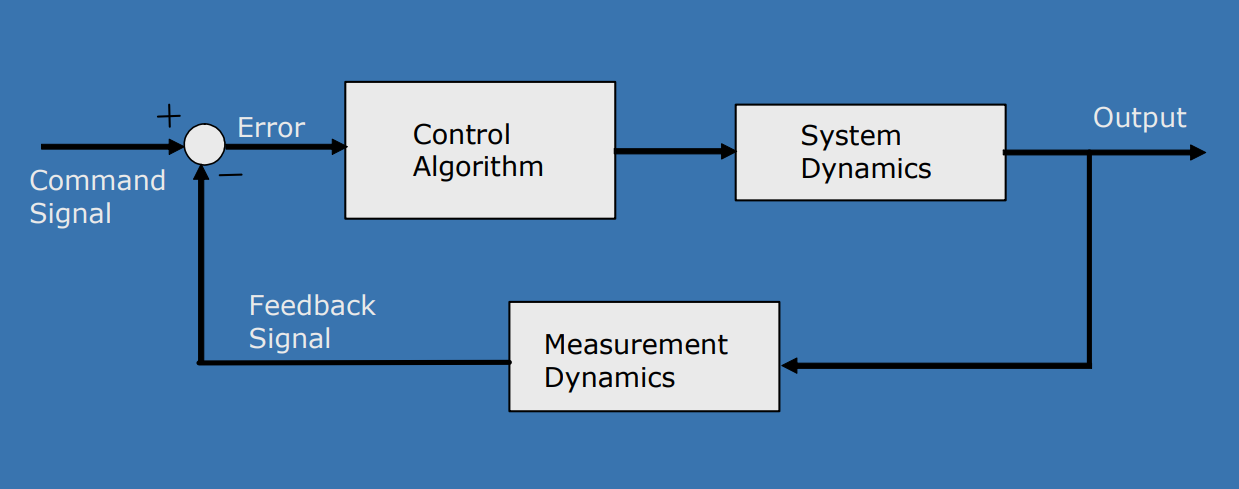
\includegraphics[width=\textwidth]{feedback-loop-block.png}
        \end{subfigure}
        \caption{State diagram of a closed-loop feedback control \cite{report:feedback-control}.}
        \label{figure:feedback-loop-block}
    \end{figure}

    \subsection{State estimation}
    \label{section:estimator}
    Sensors provide a UAV with the necessary information for flying but they usually have poor precision. As a result, although variables such as acceleration, angular velocity and absolute position can be directly measured, they are subject to noise. Furthermore, variables such as thrust and attitude angles, which are required by the UAV to fly, cannot be measured by sensors directly. State estimation is a crucial part of the feedback control loop that is used to estimate necessary variables required by the UAV directly from the sensors' data \cite{book:quan2017-state-estimators}. In the Crazyflie 2.1, two state estimators have been implemented: Complementary Filter and the Extended Kalman Filter \cite{web:stateEstimator/bitcraze}.

    \subsubsection{Complementary Filter}
    The Complementary Filter is a relatively simple attitude estimation algorithm that is implemented in the Crazyflie 2.1 based on the gradient descent algorithm by Madgwick et al. \cite{article:complementary-filter}. It accepts as input the Gyroscope, Accelerometer, and ToF (Time of Flight) measurements while outputting the attitude angles and thrust as shown in figure \ref{figure:complementary-filter-bitcraze}.

    \begin{figure}[hbt!]
        \centering
        \begin{subfigure}[b]{0.49\textwidth}
            \centering
            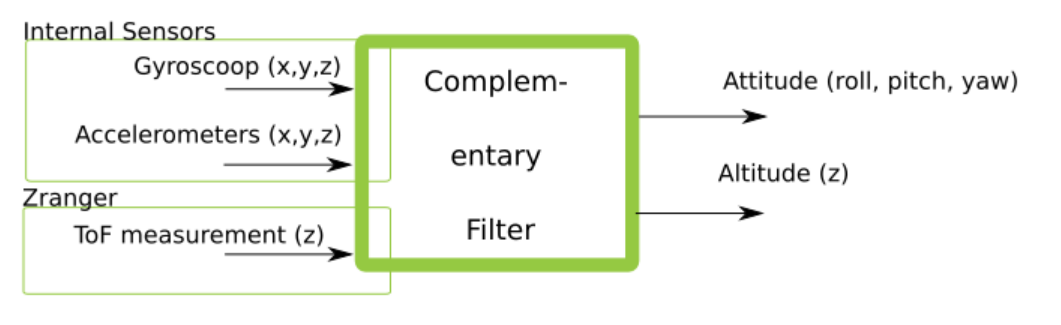
\includegraphics[width=\textwidth]{complementary-filter-bitcraze.png}
            \caption{Complementary Filter}
            \label{figure:complementary-filter-bitcraze}
        \end{subfigure}
        \begin{subfigure}[b]{0.49\textwidth}
            \centering
            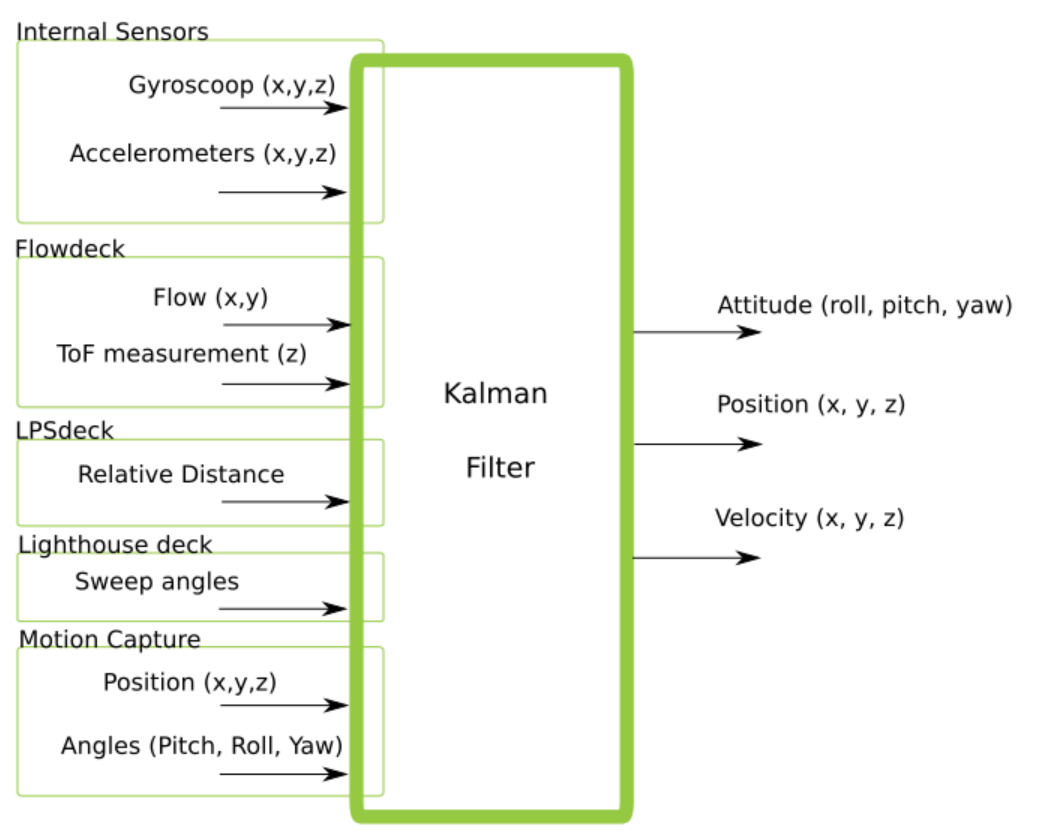
\includegraphics[width=\textwidth]{extended-kalman-bitcraze.png}
            \caption{Extended Kalman Filter}
            \label{figure:extended-kalman-bitcraze}
        \end{subfigure}
        \caption{Dataflow diagrams for state estimators used in Crazyflie 2.1 \cite{web:stateEstimator/bitcraze}}
        \label{figure:State-Estimator-bitcraze}
    \end{figure}

    \subsubsection{Extended Kalman Filter}
    The Kalman Filter also known as Linear Quadratic Estimate (LQE) is a recursive algorithm that estimates the internal state of a linear system. The algorithm uses a series of noisy measurements over time to produce estimates of unknown variables. It works in a two-step process---prediction and updation. In the prediction stage, the Kalman Filter produces estimates for the current state variables which include certain uncertainties. Then, in the updation stage, the algorithm updates these state estimates using a weighted average from the real measurements giving a higher weight to estimates that have higher certainty. The algorithm can operate in real-time and only requires the current sensor measurements and the predicted state information \cite{book:quan2017-KF}.

    A major drawback of the Kalman Filter, though, is that it assumes the noise in the measurements to have a Gaussian distribution and is only applicable to linear systems. State estimation for non-linear systems such as UAVs is considerably more difficult. Extended Kalman Filter or EKF is a non-linear version of the Kalman Filter which has been successfully applied to many nonlinear systems such as UAVs. The main principle behind the EKF is the linearization of non-linear functions by ignoring higher-order terms in the Taylor expansions (first-order linear truncation) \cite{book:quan2017-EKF}.

    In the Crazyflie, EKF accepts significantly more sensor data than the Complementary Filter and also performs better during flight. It estimates the current state of the Crazyflie in combination with a predicted standard deviation of the process noise, the measurement model, and the system model. EKF allows the possibility of full pose estimation (position/velocity + attitude) as shown in figure \ref{figure:extended-kalman-bitcraze}). EKF is preferred with external decks like the Flowdeck, the Loco Positioning deck, and the Lighthouse deck that can provide the necessary sensor information \cite{web:stateEstimator/bitcraze} required by the algorithm. In the Crazyflie, EKF has been implemented with reference to articles \cite{article:kalman-implementation-1} and \cite{article:kalman-implementation-2} by Mueller et al.
    
    \subsection{Control algorithm - PID}
    \label{section:controller}
    Control algorithms are methods that let a quadcopter set the output to the hardware of the system. They are employed in the feedback loop where sensors provide data to the estimation algorithm which sends the current estimated state to the control algorithm. The control algorithm then calculates the error between the current position and the desired setpoint to output the optimal input for the hardware (see figure \ref{figure:feedback-loop-block}).

    The Crazyflie 2.1 quadcopter software provides three different control algorithms--- PID (Proportional-Integral-Derivative), INDI (Incremental Nonlinear Dynamic Inversion), and Mellinger. The INDI and Mellinger controllers are direct applications of \cite{article:indi} and \cite{article:mellinger}. They are more recent integrations in the Crazyflie firmware and have not gone through rigorous testing. The PID control algorithm, on the other hand, has been rigorously tested and widely documented in the firmware. It is also a simple and standard algorithm and hence, we chose to rewrite it in Heptagon.

    The PID control algorithm is a linear algorithm that is widely used in robotics. It functions by calculating the error or difference between a measured output (sensors data) and a desired setpoint and adjusts the system control inputs such that the calculated error is corrected in a controlled manner in several loops to reach the desired set point to prevent sudden hiccups in the system. The PID algorithm consists of three control parameters,  P--Proportional, I–-Integral and D–-Derivative. The mathematical expression of the discrete-time PID algorithm is given by the following control function: 
            $$u_p = K_pe(t) + K_d\frac{de(t)}{dt} + K_i \int_0^te(\tau)d\tau$$ 
    Here, the term with $K_p$ determines the reaction to the current error (Proportional), the term with $K_i$ determines the reaction based on a sum of recent errors (Integral) while the term with $K_d$ responds to the rate at which the error has been changing (Derivative) \cite{article:pid-controller-IIJEM}.

    The PID controller implemented in Crazyflie is also called a Cascaded PID controller. This is because the PID controller is linearly applied to the input four times to evaluate the final output. The cascaded PID controller takes the desired set-point as one of the inputs and passes it through the \code{Position}, \code{Velocity}, \code{Attitude}, and \code{AttitudeRate} PIDs to eventually determine the desired control power (see appendix \ref{appendix:previous-block-diagram} for a high-level overview of the cascaded PID controller). The power output is handled by the power distribution of the motors to eventually achieve the desired setpoint.
    
\section{Contributions}
    \label{section:contributions}
    In the previous section, the theoretical frameworks required to understand the contributions in this thesis which are to implement the Crazyflie's C code in Heptagon were explained. Initially, this thesis was supposed to begin by implementing the cascaded PID controller as suggested by the  preceding report \cite{report:cse303-report}. However, as the thesis began, the cascaded PID controller as well as the power distribution section of the feedback control loop had already been implemented by our colleagues. Consequently, we began with integrating these implementations in the original Crazyflie firmware followed by their verification through flight tests. Subsequently, we focused on implementing the Complementary Filter, the led sequence FreeRTOS task, and the Kalman Filter in Heptagon.
    
    \subsection{Cascaded PID controller}
    The cascaded PID controller had been implemented and debugged individually for the \code{Position}, \code{Velocity}, \code{Attitude}, and \code{AttitudeRate} PIDs by our colleagues. We started by combining these individual PIDs into a single node \textFunc{controller\_pid} which is similar to the cascaded PID controller in the original firmware (represented by the controller block in appendix \ref{appendix:previous-block-diagram}). To replace the original cascaded PID controller with the \textFunc{controller\_pid} node implemented in Heptagon, additional C functions were needed to respect Heptagon's calling conventions \cite{report:heptagon_manual}. The method to do this is explained in the following subsection.

    \subsubsection{Integrating Heptagon generated C code}
    \label{section:integrate-hept-c-code}
    All the nodes for the PID controller were written in the \code{libel.ept} file (\code{.ept} is extension for Heptagon). Therefore, according to the Heptagon convention, the C code generated using \code{make} was placed in the directory called \code{Libel\_c} (first letter is uppercase). In this directory, a file \code{Libel.c} was created that contained two functions for each node (let's say \textFunc{quaternion}) as follows:
    \begin{enumerate}
        \item \code{void} \quad \textFunc{Libel\_\_quaternion\_reset(Libel\_\_quaternion\_mem* self);} \\\\
            The \code{reset} C function takes an argument \code{self} and is used to set all the variables used in the \textFunc{quaternion} node (contained in the \code{Libel\_\_quaternion\_mem} struct in the generated C code) to zero.
        \item 
            \begin{tabbing}
                \code{void} \quad \textFunc{Libel\_\_quaternion\_step(} \\
                \code{\quad\quad Libel\_\_quaternion \quad input\_q}\\
                \textFunc{\quad \quad Libel\_\_quaternion\_out* \_out,}\\
                \textFunc{\quad \quad Libel\_\_quaternion\_mem* self}\\
                \code{);}
            \end{tabbing}
            The \code{step} C function takes in the input argument (\textFunc{input\_q}) of the type (\textFunc{Libel\_\_quaternion}) to the node \textFunc{quaternion}. It also inputs the \code{\_out} and \code{self} struct pointers. The \code{self} variable points to all the variables of the \textFunc{quaternion} node in the generated C code. The \code{\_out} variable points to the following struct that contains the output (\textFunc{output\_q}) of the type (\textFunc{Libel\_\_quaternion}) from the \textFunc{quaternion} node:
            \begin{tabbing}
                \code{typedef struct \{}\\
                \code{\quad Libel\_\_quaternion \quad output\_q;}\\
                \} \quad \code{Libel\_\_quaternion\_out;}
            \end{tabbing}
    \end{enumerate}
    The input and output types (\textFunc{Libel\_\_$t_1$, \dots, Libel\_\_$t_n$}) and (\textFunc{Libel\_\_$t_1^{'}$, \dots, Libel\_\_$t_n^{'}$}) respectively are unique to the \code{Libel.c} file and used by the Heptagon-generated C code. Hence, to communicate with it, the data from the original C implementation needs to be converted into the data types of the Heptagon-generated C code. This can be done using functions like the ones given in listing \ref{listing:Heptagon-c-code-conversion} where data is converted from the original types to the Heptagon types and vice-versa.

    \bigskip
    \begin{lstlisting}[caption={C functions to convert Heptagon C code into original code and vice-versa}, label={listing:Heptagon-c-code-conversion}, language=C]
void quaternion_to_heptagon(const quaternion_t *in, Libel__quaternion *out) {
    out->qx = in->x;
    out->qy = in->y;
    out->qz = in->z;
    out->qw = in->w;
}
void heptagon_to_quaternion(const Libel__quaternion *in, quaternion_t *out) {
    out->x = in->qx;
    out->y = in->qy;
    out->z = in->qz;
    out->w = in->qw;
}   \end{lstlisting}
    \bigskip

    The function \textFunc{quaternion\_to\_heptagon} converts a struct \code{quaternion\_t} used in the original firmware to the struct \code{Libel\_\_quaternion} that is recognized by \code{step} function in the Heptagon generated C code, and vice-versa for \textFunc{heptagon\_to\_quaternion} C function. These functions can be used to transform the data types of the original input and output to those accepted by the Heptagon generated C function  \textFunc{Libel\_\_quaternion\_step} as shown in listing \ref{listing:Heptagon-c-code-integration}. Lines \ref{line:hept-def-start}-\ref{line:hept-def-end} declare the \code{Libel} struct variables needed by the Heptagon-generated C code. Line \ref{line:heptagon-convert} changes the original quaternion input (\code{quaternion\_t}) to the one accepted by the \code{step} function (\code{Libel\_\_quaternion\_step}), and line \ref{line:heptagon-output-out} converts the output (\code{output\_q}) from the \code{out} struct which is of the type \textFunc{Libel\_\_quaternion} to the original quaternion type (\code{quaternion\_t}). Eventually, the original quaternion (\code{original\_q}) points to the output from the \textFunc{quaternion} node implemented in Heptagon and can be used further in the original firmware.

    \bigskip
    \begin{lstlisting}[caption={Calling \textFunc{quaternion} node from original firmware}, label={listing:Heptagon-c-code-integration}, language=C]
static Libel__quaternion hept_q;                    $\label{line:hept-def-start}$
static Libel__quaternion_mem quaternion_mem;
static Libel__quaternion_out quaternion_out;        $\label{line:hept-def-end}$

void modify_quaternion(quaternion_t *original_q)
{
    quaternion_to_heptagon(original_q, &hept_q);             $\label{line:heptagon-convert}$
    Libel__quaternion_step(hept_q, &quaternion_out, &quaternion_mem);
    heptagon_to_quaternion(&controller_out.output_q, original_q);     $\label{line:heptagon-output-out}$
}   \end{lstlisting}
    \bigskip

    \subsubsection{Final result}    
    After integrating the \textFunc{controller\_pid} Heptagon node using appropriate C functions, the quadcopter was run through flight tests to verify the correctness of the Heptagon implementation. The quadcopter did not fly as expected initially, but after some modifications to the initialization for the \code{reset} function of the \textFunc{controller\_pid} node, the quadcopter flew as expected. Figure \ref{figure:pid-controller-block} show the dataflow diagram that can be derived from the Heptagon implementation of the cascaded PID controller. The diagram clearly shows how the data for specific variables flows through the different PIDs in a synchronous manner.

    \begin{figure}[hbt!]
        \centering
        \begin{subfigure}[b]{0.99\textwidth}
            \centering
            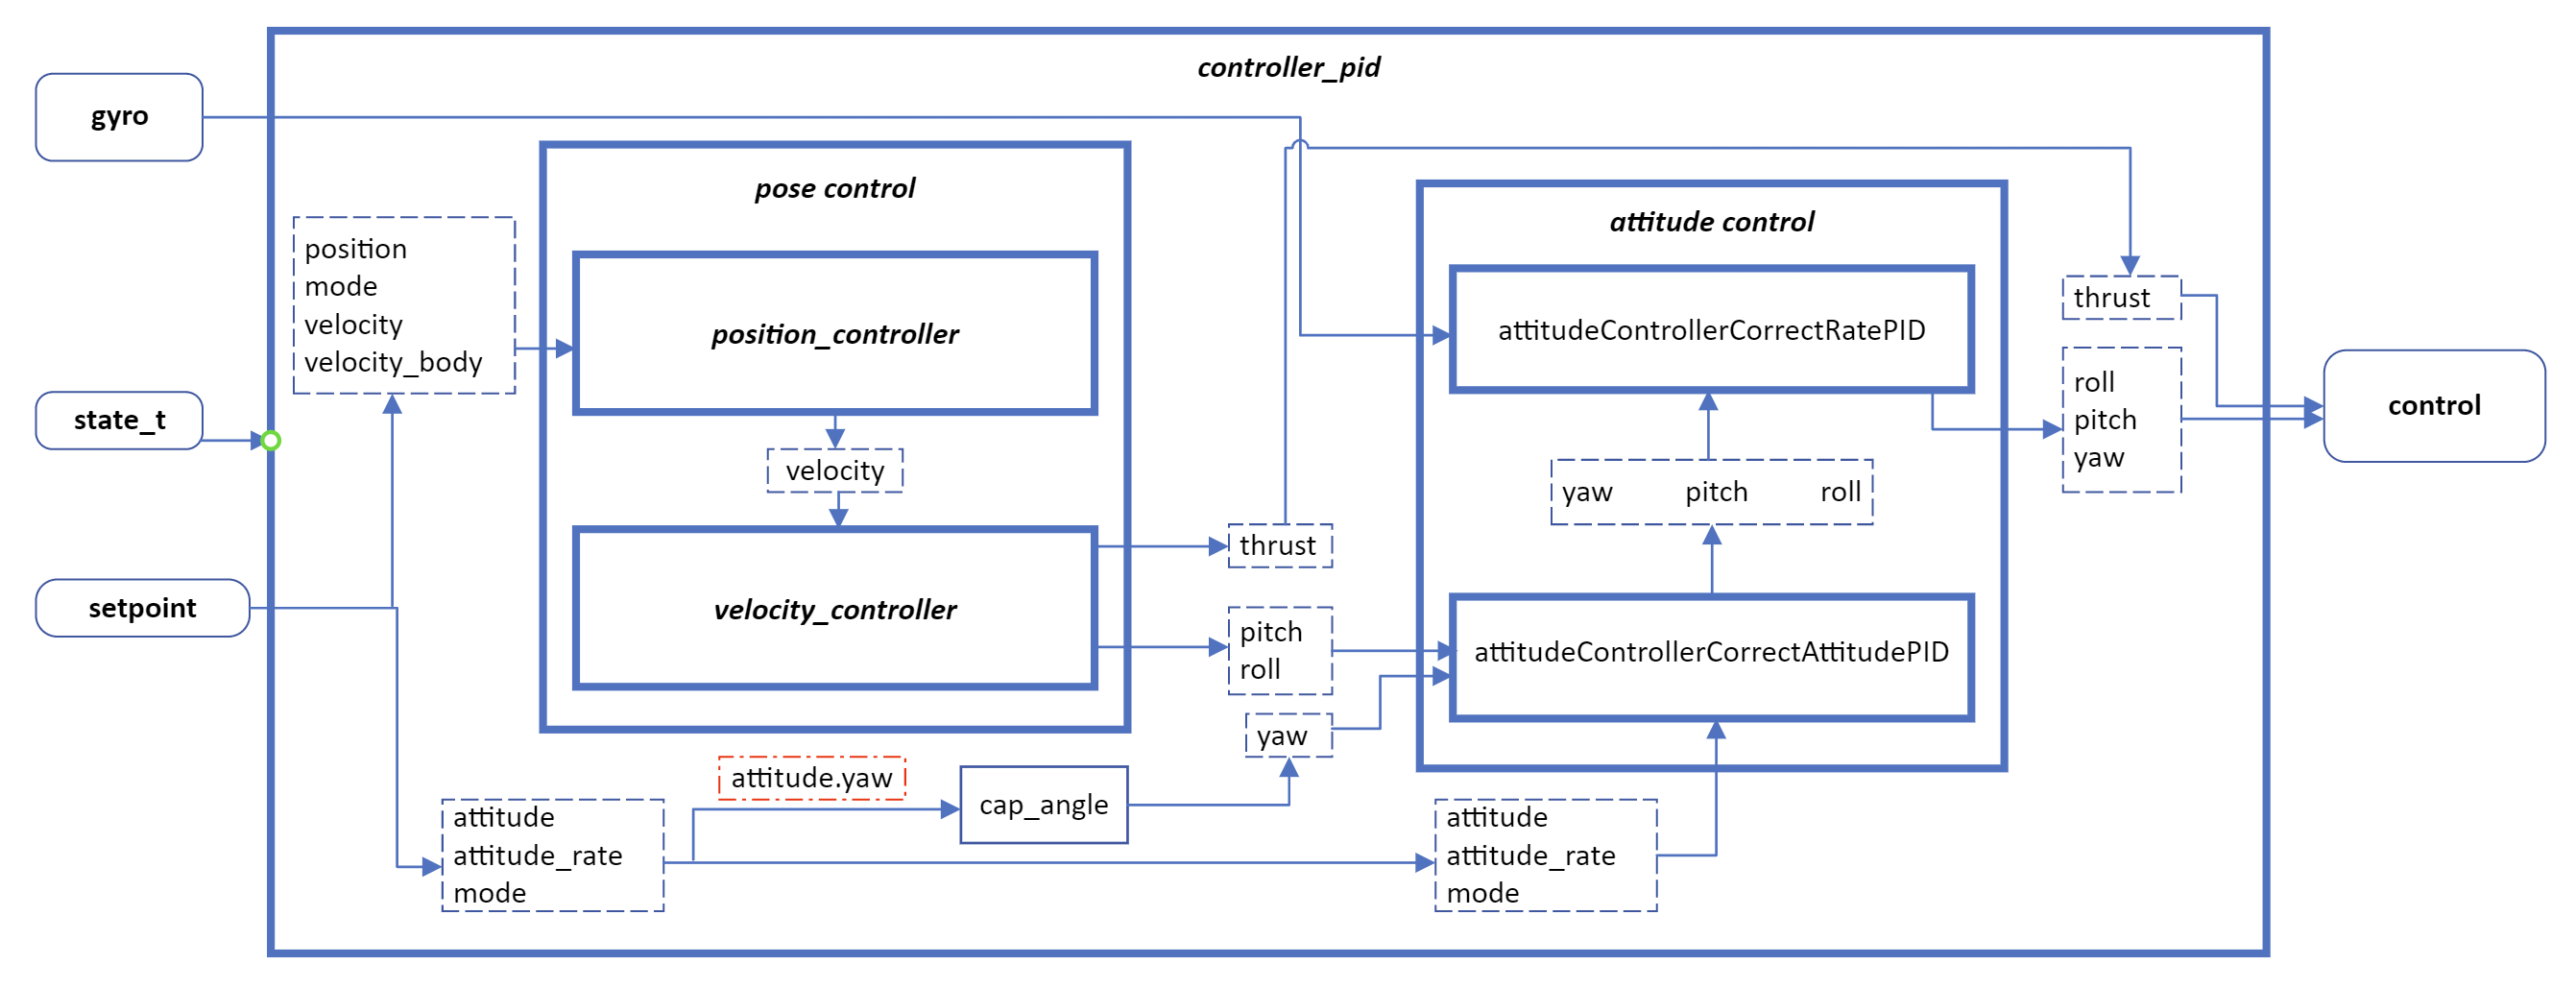
\includegraphics[width=\textwidth]{pid-controller-block.png}
        \end{subfigure}
        \caption{Dataflow diagram for PID controller from Heptagon implementation.}
        \label{figure:pid-controller-block}
    \end{figure}

    \subsection{State estimator - Complementary Filter}
    After the cascaded PID controller, we focused on writing the Complementary Filter in Heptagon. The Complementary Filter is implemented across three different files in the original firmware. The algorithm passes redundant variables across several C functions and uses static variables in each file making it difficult to follow its dataflow. Our Heptagon implementation, on the other hand, defines the Complementary Filter across $6$ main nodes and $6$ memoryless functions (defined as \textFunc{fun} in Heptagon) which is simpler to understand visually. It was compiled with the Heptagon compiler and integrated into the firmware by replacing the original C implementation with the Heptagon-generated C code. The integrated code, though, encountered issues in the initial flight tests which started a lengthy debugging process explained in the following subsections.

    \subsubsection{Debugging process}
    The Crazyflie firmware allows debugging through the \textFunc{consolePrintf()} or \textFunc{DEBUG\_PRINT()} functions which print output directly on the Crazyflie PC client \cite{software:crazyflie-clients-python} that is used to connect the Crazyflie. This method for debugging the UAV, though, is too time-consuming and complicated. The entire code needs to be rebuilt for any change made in the firmware, then this code must be flashed to the UAV, and the UAV should be reconnected with the PC client where the output is displayed. An alternative debugging approach is to compare the Heptagon implementation directly with the original implementation without running the code on the UAV. The Complementary Filter only takes in the sensor data as input and outputs the estimated state. Essentially, a custom testing environment can be created in C that runs the original estimator code (as the reference) and the Heptagon implementation side-by-side by passing the same input sensors data and comparing the difference in the resultant output states of the two implementations.

    To run the custom testing environment, we needed the actual sensor data. For this, we used the \code{cflib} library written in Python and provided by Bitcraze to communicate with the Crazyflie family of quadcopters \cite{software:crazyflie-clients-python}. This Python library allows the Crazyflie to send real-time flight data to a PC. The maximum data size that can be sent is $30$ bytes out of which four bytes are used for the block id and the timestamp (see appendix \ref{software-reference:crazyflie-max-log-len}). The Complementary Filter algorithm accepts four sensor data variables---gyro, acc, baro, and tof---all of which are three-dimensional arrays that are logged as $32$-bit integers (four bytes) on the original firmware. Hence, each sensor variable is $12$ bytes long. The total data that we need to send from the Crazyflie thus, amounts to a total of $48$ bytes. Therefore, to log all four three-dimensional sensor data variables simultaneously, we decided to convert each value into a $16$-bit floating point number ($24$ bytes in total) with the "FP16" data type \cite{software:crazyflie-FP16} at the cost of losing precision. These values were then stored in a text file that was used to feed data into the custom testing environment over several runs. Eventually, the testing environment instantly highlighted the discrepancies in the output generated by the two estimator implementations when fed with the sensor data. Through the debugging, three main issues were found in the Heptagon code. One was a logical bug while the other two were more complicated and are discussed in the following subsections.

    \subsubsection{Bug in Heptagon compiler}
    \label{section:bug-in-compiler}
    One of the discrepancies highlighted by the debugging was in the z-component of the acceleration vector (acc) of the state variable (see appendix \ref{appendix:previous-block-diagram} for the state data structure). This was bizarre because, for certain inputs, this specific variable was not even accessed (as intended by the code and confirmed through debug prints) but was still being modified in the output. The exact problem seemed to arise in lines \ref{line:acc_z_bug_start}-\ref{line:acc_z_bug_end} of the code in listing \ref{listing:Heptagon_bug}. This piece of code, theoretically, only assigns a new record to the state variable, but in the debugging runs it seemed to modify the value of \textFunc{st\_acc} (line \ref{line:acc_z_bug_end}) by setting it to that of \textFunc{st\_position} (line \ref{line:st-position}). To understand this behaviour, we inspected the C code generated for the node. On careful analysis, it was found that the compiler was switching the values \textFunc{st\_position\_z} and \textFunc{st\_acc\_z}. This was eventually confirmed to be a bug in the Heptagon compiler \cite{software:heptagon-issue} which was generated from the \code{memalloc} optimization. Hence, for the rest of the thesis, we turned off the \code{memalloc} optimization. With the optimization switched off, Heptagon compiled the C code correctly and this part of the node behaved as expected.

    \begin{lstlisting}[caption={Buggy Heptagon node}, label={listing:Heptagon_bug}, language=C]
node estimator_complementary(sensor: sensor_data_est)
returns (st : state_t);

$ \text{... (See appendix \ref{appendix:estimator-node})}$

    last st_attitude_this: attitude = {roll = 0.0; pitch = 0.0; yaw = 0.0};
    last st_attitude_quat_this: quaternion = {qw = 1.0; qx = 0.0; qy = 0.0; qz = 0.0};
    last st_acc_z: float = 0.0;
    last st_position_z: float = 0.0;
    last st_velocity_z: float = 0.0;

$ \text{... (See appendix \ref{appendix:estimator-node})}$

    st = {  st_attitude = st_attitude_this; $\label{line:acc_z_bug_start}$
            st_attitude_quat = st_attitude_quat_this;
            st_position = {x = 0.0; y = 0.0; z = st_position_z};    $\label{line:st-position}$
            st_velocity = {x = 0.0; y = 0.0; z = st_velocity_z};
            st_acc = {x = 0.0; y = 0.0; z = st_acc_z}}; $\label{line:acc_z_bug_end}$
tel
\end{lstlisting}
    \bigskip

    \subsubsection{Floating point numbers and fast inverse square root}
    The second major discrepancy in the Heptagon code was related to error propagation. In the first few hundred iterations of the control loop, the output variables from the state estimators differed by an order of $1e-5$, but because these errors were propagated over time, the estimation algorithm started integrating them to reach an order of $1$. This error margin is too big and significantly destabilizes the quadcopter. A thorough debugging analysis revealed that this error was introduced for two reasons. 

    The first reason is compiler-based. The definition of $pi$ in the main firmware code is defined to be $M\_pi = 3.14159265358979323846$, but in the C code generated by Heptagon, this value is truncated to $6$ decimal places where $M\_pi = 3.141592$. This discrepancy creates differences in the final output of the two estimator implementations to the order of $1e-14$ which is confirmed by running specific equations involving $pi$ and shown in figure \ref{figure:invSqrt}. In the figure,  \code{reference} is the output from the original firmware code while \code{Heptagon} is the output from the Heptagon implementation where $qw$, $qx$, $qy$, and $qz$ are the four quaternion variables. It can be observed that the readings for $qy$ and $qz$ are different in the last two hexadecimal digits due to the difference in values of $pi$. Although insignificant in itself, this difference becomes important for the second issue.

    \begin{figure}[hbt!]
        \centering
        \begin{subfigure}[b]{0.99\textwidth}
            \centering
            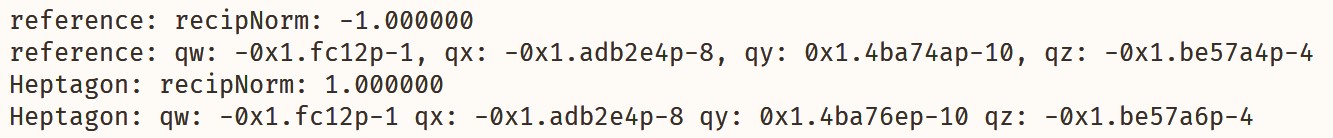
\includegraphics[width=\textwidth]{invSqrt_discrepancy.jpg}
        \end{subfigure}
        \caption{Discrepancy in readings from fast inverse square root function.}
        \label{figure:invSqrt}
    \end{figure}

    The second issue is algorithm specific. The estimation algorithm normalizes the quaternions using the fast inverse square root algorithm \cite{web:wiki-invSqrt} given in listing \ref{listing:fast-invsqrt} which exploits low-level bit hacking techniques that are only available in C. Heptagon cannot perform such manipulations and hence the algorithm was defined and used as an external function (section \ref{section:syntactic-extensions}). Still, the same C code for the algorithm generates different normalized outputs for the original and Heptagon implementations as shown in figure \ref{figure:invSqrt}. Here, \code{recipNorm} is the normalized output from the two implementations. The fascinating aspect of this output is that a square root approximating algorithm turns $1.0$ to $-1.0$ for an almost negligible change in the input (order of $1e-14$). This points to an overflow of the sign bit and seems to arise from lines \ref{line:weird-stff-starts}-\ref{line:weird-stff-ends} whose behaviour can change for different architectures. The build environment used by the machine with the testing environment was a $64$-bit architecture, hence we decided to use $32$-bit architecture-specific C libraries instead to build the testing environment. In doing so, the algorithm gave similar results for both implementations with an error to an order of $1e-6$. The Crazyflie uses a $32$-bit architecture hence, the error in the calculations there would be to an order of $1e-6$ which is under acceptable limits.

    \bigskip
    \begin{lstlisting}[caption={Fast inverse square root original C Implementation (see appendix \ref{software-reference:invSqrt})}, label={listing:fast-invsqrt}, language=C]
float Q_rsqrt( float number )
{
    long i;
    float x2, y;
    const float threehalfs = 1.5F;

    x2 = number * 0.5F;
    y  = number;
    i  = * ( long * ) &y;                       // evil floating point bit level hacking $\label{line:weird-stff-starts}$
    i  = 0x5f3759df - ( i >> 1 );               // what the fuck? 
    y  = * ( float * ) &i;                      $\label{line:weird-stff-ends}$
    y  = y * ( threehalfs - ( x2 * y * y ) );   // 1st iteration
//	y  = y * ( threehalfs - ( x2 * y * y ) );   // 2nd iteration, this can be removed

    return y;
}    \end{lstlisting}

    \subsubsection{Final result}
    After fixing the bugs, the final implementation was integrated into the original firmware and tested through flight tests. The flight results were similar to those observed with the original implementation and hence the Heptagon implementation for the Complementary Filter was verified. This Heptagon implementation can be modelled in a dataflow diagram as shown in figure \ref{figure:compl_estimator}. The diagram gives a clear specification of the Complementary Filter algorithm that is hard to generate from the original firmware. In the algorithm, the ToF measurements come from the ZRanger deck. If the deck is not available, as in our case, the ToF input and equations can be removed from the node.

    \begin{figure}[hbt!]
        \centering
        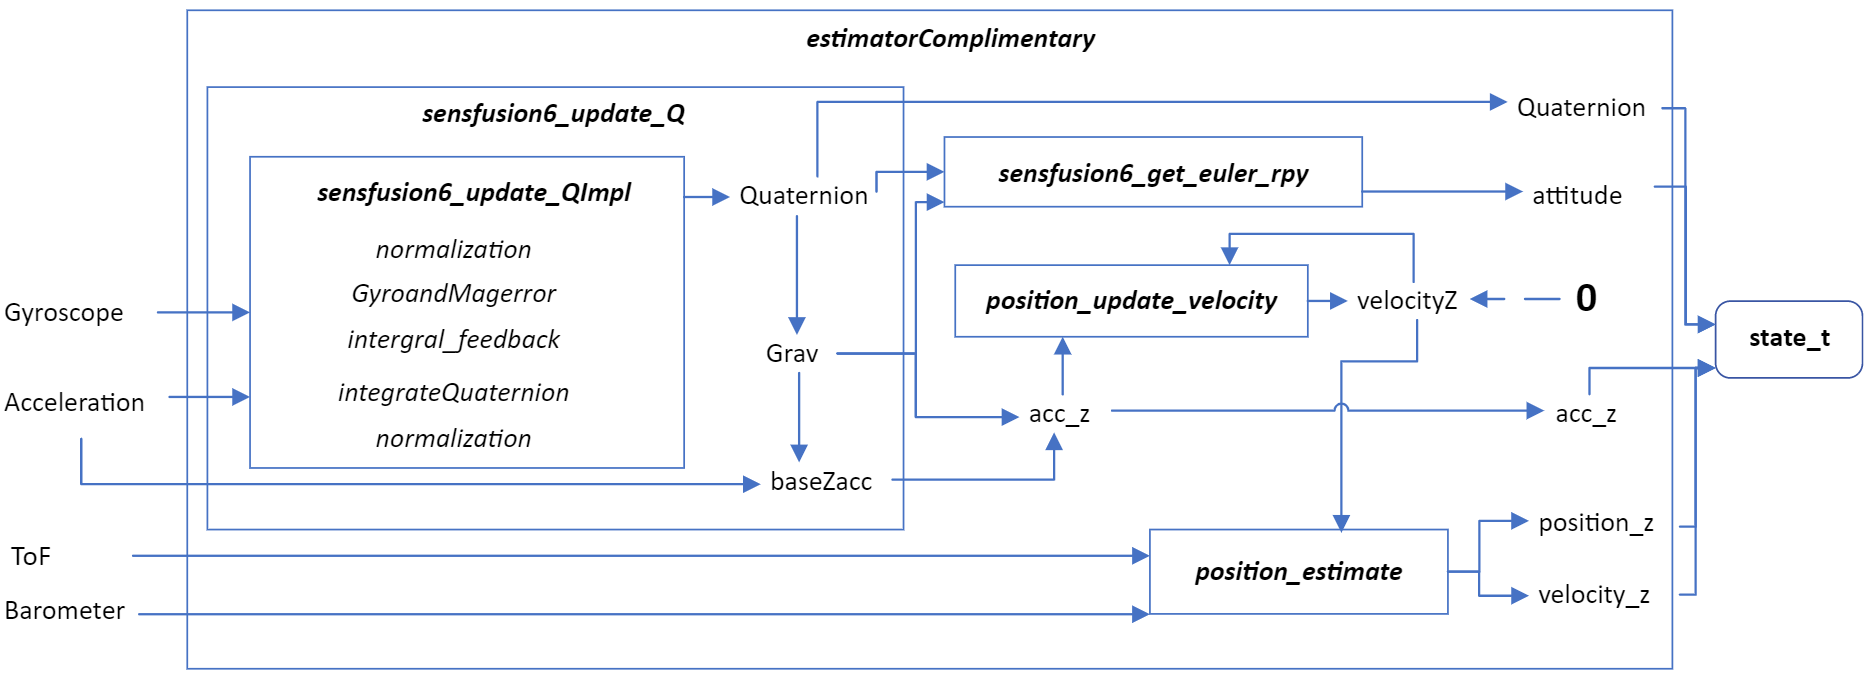
\includegraphics[width=0.99\textwidth]{compl_estimator_block.png}
        \caption{Block diagram for Complementary Filer implemented in Heptagon.}
        \label{figure:compl_estimator}
    \end{figure}

    \subsection{Merging the controller and the estimator}
    \label{section:controller-estimator-merging}
    As explained in section \ref{section:integrate-hept-c-code}, to integrate the Heptagon generated C code in the original firmware, data must be converted between different types in the original firmware as it is sent to and from the Heptagon code. The estimator and the controller have now been converted to Heptagon but they do not run one after the other as the high-level commander function is called between them (see appendix \ref{appendix:previous-block-diagram}). Therefore, the inputs and outputs to the Heptagon nodes are converted two times with no direct communication between them. This is undesirable as the goal of the thesis is to implement the maximum amount of the original firmware in Heptagon and exploit its synchronous capabilities to define clear semantics of the program while the compiler takes care of the low-level implementation details.

    On a careful investigation of the feedback control loop, it was observed that the commander runs at a frequency of $1000Hz$ (period $=1ms$) and essentially returns the desired setpoint to the controller that the quadcopter wants to achieve. We decided to run the commander after the controller which meant that the controller would receive the desired setpoint with a delay of $1ms$. The commander itself updates the setpoint with a frequency of $100Hz$ or every $10ms$ (appendix \ref{software-reference:commander-freq}), hence, the delay of $1ms$ should hypothetically not make any noticeable difference in the quadcopter's flight. For confirmation, when the quadcopter was run through flight tests, the reorganized code did not have any observable change in the quadcopter's flights. Therefore, the estimator (Complementary Filter) and the controller (cascaded PID) were merged in the \textFunc{combined\_estimator\_controller} node. This node runs the estimator and the controller synchronously giving simple and clear semantics for the program as shown in the dataflow diagram in figure \ref{figure:combined-estimator-controller}.

    \begin{figure}[hbt!]
        \centering
        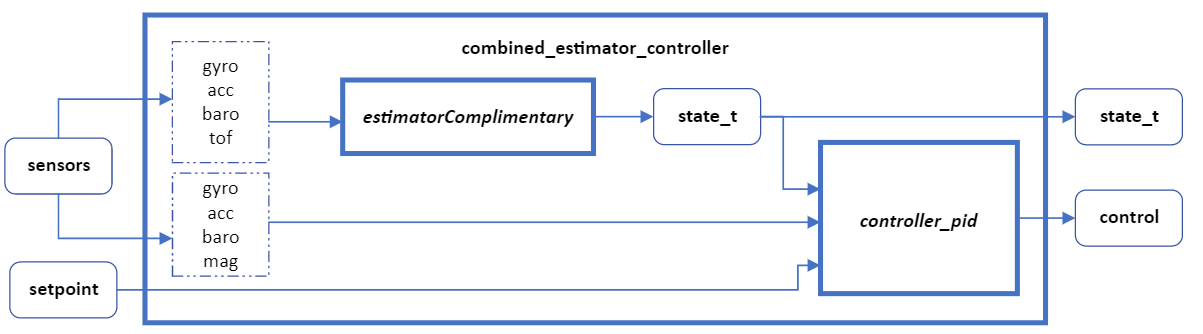
\includegraphics[width=0.99\textwidth]{combined-estimator-controller.png}
        \caption{Block diagram for combined estimator (complementary) and controller (PID) node.}
        \label{figure:combined-estimator-controller}
    \end{figure}

    \subsection{Led sequence FreeRTOS task integration}
    \label{section:ledseq-task}
    After implementing the feedback control loop in Heptagon, we focused our attention to FreeRTOS tasks. The non-deterministic nature of the preemptive scheduler implemented in Crazyflie makes it hard to define clear semantics for the behaviour of tasks in the program as pointed out in section \ref{section:preemptive-scheduler}. Figure \ref{figure:timeflow_readings} shows two possible ways of how a pair of tasks---stabilizer and led\_seq---may behave. Here, the stabilizer task is a high-priority task that is released from the Blocked state to the Ready state every $1$ms while the led\_seq task is a lower priority one which is almost always in the Ready state. In figure \ref{figure:timeflow_reading1}, the led\_seq task gets enough execution time but in figure \ref{figure:timeflow_reading2} it does not. With the current C implementation, it is hard to argue which of these behaviours is correct. By replacing the tasks implemented in Crazyflie with Heptagon nodes, which run deterministically, a clear specification for the UAV can be obtained to better answer the question.

    Crazyflie has $37$ different tasks defined in its firmware. A majority of these tasks are for external expansion decks \cite{web:expansion-decks} that may be added to the Crazyflie for better performance. Out of all the possible tasks, appendix \ref{appendix:FreeRTOS-tasks} gives the list of $13$ tasks running on our model of the Crazyflie with their individual priorities. Out of these tasks, the \code{ledseqCmdTask} is responsible for running the led sequence for the quadcopter. It is a relatively simple task and visually easier to debug. Therefore, we first chose to implement the \code{ledseqCmdTask} as a Heptagon node---\textFunc{ledseq\_task}---and see how the FreeRTOS tasks may be replaced.

    \subsubsection{Initial approach}
    The stabilizerTask has the highest priority of $5$ (appendix \ref{software-reference:stabilizer-task-priority}) of all the tasks in Crazyflie. This task runs the main feedback control loop of the UAV at a frequency of $1000Hz$ (appendix \ref{software-reference:stabilizer-freq}). In the initial approach, we decided to integrate the \textFunc{ledseq\_task} Heptagon node outside the stabilizerTask and to run it right after the execution of the stabilizerTask at a frequency of $500Hz$ as shown in figure \ref{figure:timeflow_readings}. With this approach though, the LEDs remained static and never blinked when the quadcopter was tested. After a debugging analysis, it was found that the Heptagon node was not being run by the processor. The reason is that when the Heptagon node was integrated into the Crazyflie firmware, the declaration of the FreeRTOS \code{ledseqCmdTask} was removed. Doing this removed any access the scheduler had to dynamically change the LEDs once the quadcopter was initialized. This is because the FreeRTOS scheduler always runs some task on the processor, and if no user-defined task is being run, it automatically runs the idle task as explained in section \ref{section:idle-task}. Essentially, once the scheduler is initiated using the \textFunc{vTaskStartScheduler()} FreeRTOS API function, the processor only runs the code defined inside FreeRTOS tasks as they are delegated by the scheduler. Therefore, with the current approach, the \textFunc{ledseq\_task} Heptagon node was out of reach for the scheduler and as good as dead code.

    \begin{figure}[hbt!]
        \centering
        \begin{subfigure}[b]{0.98\textwidth}
            \centering
            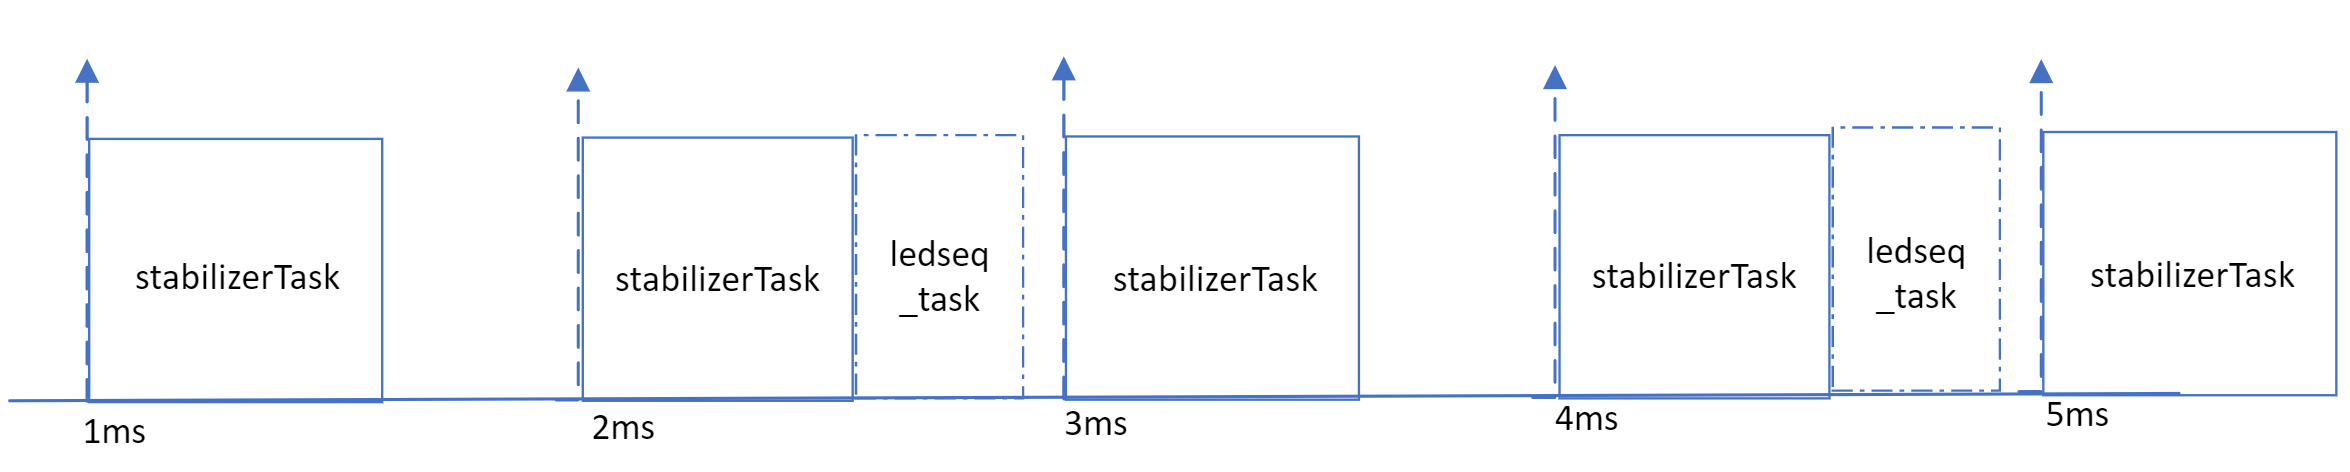
\includegraphics[width=\textwidth]{timeflow1.png}
            \caption{Case when implementation is within $1ms$ bound.}
            \label{figure:timeflow_reading1}
        \end{subfigure}
        \begin{subfigure}[b]{0.98\textwidth}
            \centering
            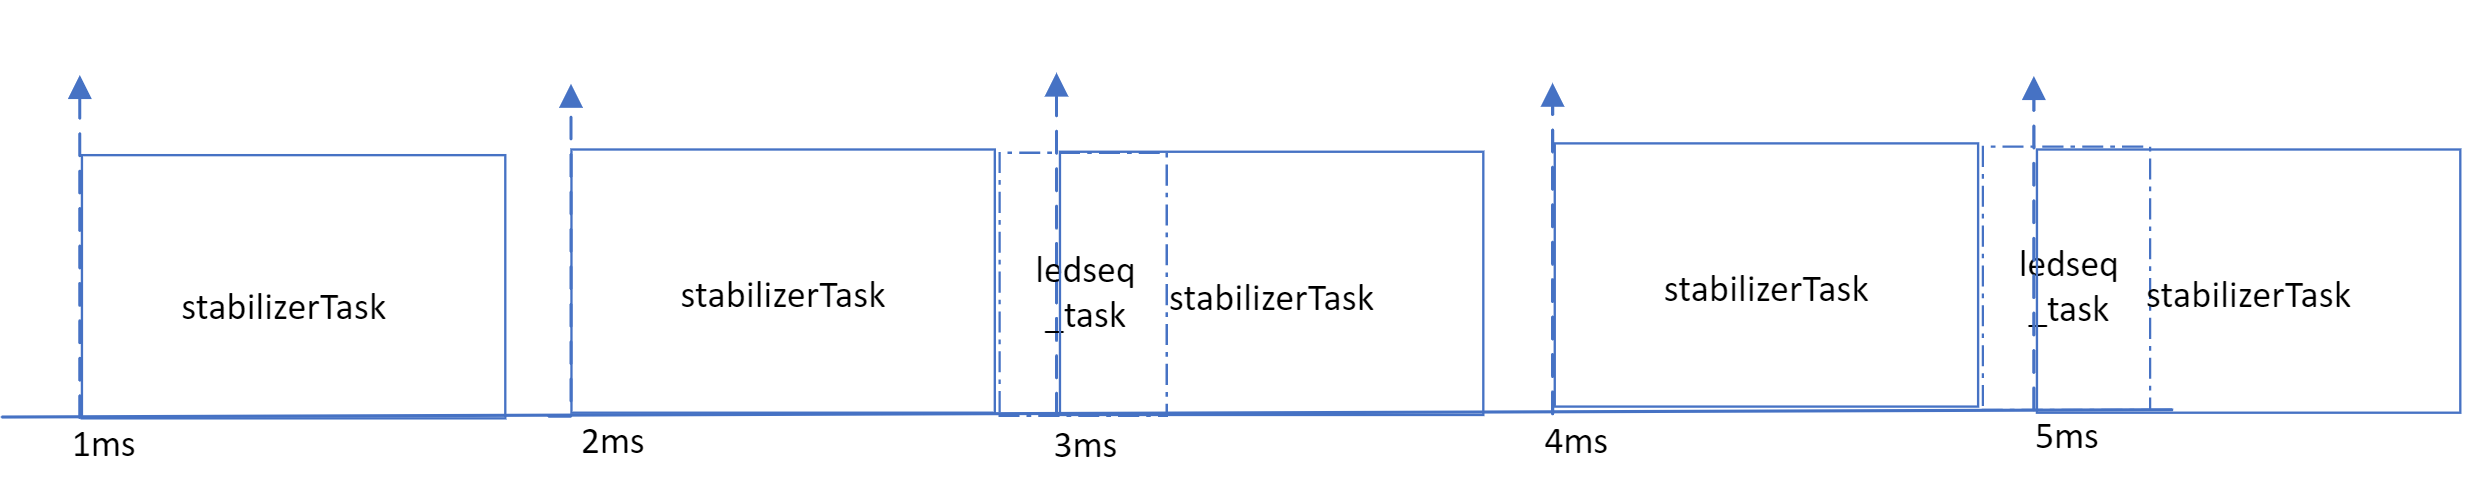
\includegraphics[width=\textwidth]{timeflow2.png}
            \caption{Case when implementation overshoots $1ms$ bound.}
            \label{figure:timeflow_reading2}
        \end{subfigure}
        \caption{stabilizerTask and \code{ledseq\_task} Heptagon node execution time.}
        \label{figure:timeflow_readings}
    \end{figure}

    \subsubsection{Modified approach}
    In the modified approach, the \textFunc{ledseq\_task} was integrated to run at the end of the stabilizerTask. Essentially, it was run after executing the entire feedback control loop just like in the initial approach but inside the stabilizerTask instead of outside. Using this approach though, the LEDs switched on but did not blink as the code intended. This happened due to the "retinal persistence" effect where an image stays on the retina for some time even after the original stimulus is modified. The \textFunc{ledseq\_task} was running at a frequency of $500Hz$ and thus effecting retinal persistence. On changing the frequency to $10Hz$ (period $=100ms$), the LEDs blinked exactly as expected by the Heptagon node.

    The modified Heptagon implementation used state machines (section \ref{section:syntactic-extensions}) to switch the LEDs on and off. State machines gave simple-to-understand semantics for implementing the led sequence as represented by the dataflow diagram in figure \ref{figure:led_seq}. In the diagram, straight lines represent the flow of data between nodes and curved lines represent the switching of states. The main \textFunc{ledseq\_task} Heptagon node does not take any input but returns a record of all the LEDs on the UAV (six) where they are either on (true) or off (false). This node calls the \textFunc{led\_seq\_everyn} node that modifies the state of the LEDs at a frequency of $10Hz$. This node further calls \textFunc{led\_on\_every\_n\_tick} node which turns a led on (true) after every $n$ iterations. In the current implementation, $n=2$ so, the led is switched on at a frequency of $5Hz$ where it alternates on and then off every $100ms$ each. In the \textFunc{led\_seq\_everyn} node, the 'switched on' led is cyclically transferred between all six LEDs every 20 clock cycles ($0.5Hz$ or period $=2s$). As a result, each led blinks on and off at a frequency of $5Hz$ for two seconds in a never-ending cycle.

    \begin{figure}[hbt!]
        \centering
        \begin{subfigure}[b]{0.99\textwidth}
            \centering
            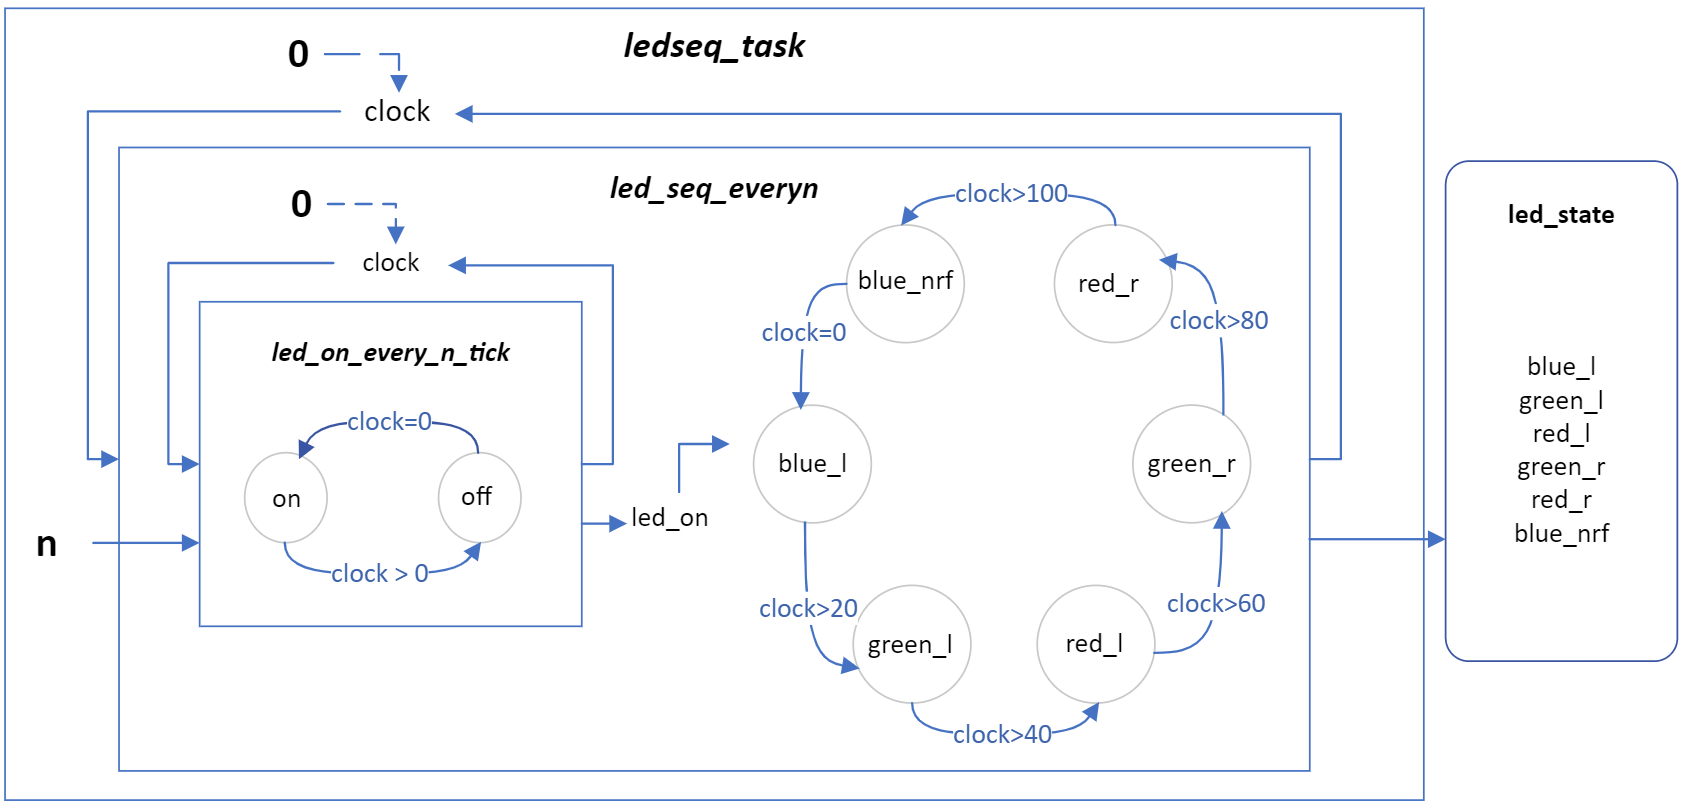
\includegraphics[width=\textwidth]{led_seq_block.png}
        \end{subfigure}
        \caption{Dataflow diagram for led sequence implemented in Heptagon.}
        \label{figure:led_seq}
    \end{figure}

    \subsubsection{Timing aspect}
    After integrating the Heptagon node for the LEDs, it was important to understand the timing aspect of the program. Timing is crucial for any embedded system where it is essential that the software and the hardware behave exactly how they are expected to by the semantics. The stabilizerTask is the most important task in the Crazyflie as it runs the main feedback control loop that instructs how the quadcopter must fly. In the initial approach, the Heptagon node was integrated outside of the feedback control loop, and hence, the timing of the loop was not modified. In the modified approach, though, the Heptagon node was integrated inside the stabilizerTask. This integration would naturally alter the task's timing as it would now run for longer than before. In this scenario, it becomes essential to determine if this modification significantly alters the execution time of the feedback control loop (stabilizerTask) where it may overshoot its originally intended run-time of $1ms$ as shown in figure \ref{figure:timeflow_reading2}.

    To investigate the timing aspect, we decided to run the modified code on the UAV and log the raw run-time of different sections of the stabilizerTask running the feedback control loop. In the Crazyflie, the smallest measurable time interval for the FreeRTOS system clock is defined to be $1ms$ because \textFunc{configTICK\_RATE\_HZ\_RAW} is defined as $1000$ (appendix \ref{software-reference:tick-rate}), but Crazyflie's feedback control loop itself runs every $1ms$ and hence we needed a more accurate timer. For this, we used the \textFunc{usecTimestamp()} function implemented by STM32F405 micro-controller that measures time to an accuracy of $1\mu s$. We used this function to log $32-$bit floating point numbers for the raw run-time of the modified stabilizerTask by dividing it into three sections that were recorded in different variables.

    In the first recorded section, the  stabilizerTask waits to receive data from the sensors and is released from the Blocked state at a frequency of $1000Hz$. In the second recorded section, once the sensor's data is ready and the task enters the Running state (because it has the highest priority and preempts any other task), the task executes one iteration of the feedback control loop. In the third recorded section, the task executes the \textFunc{ledseq\_task} Heptagon node. The running time for these three sections was recorded in three separate variables that have been plotted in figures \ref{figure:usec_readings1} and \ref{figure:usec_readings2}. Figure \ref{figure:usec_readings1} shows the data when the Crazyflie was in a static non-flying state. Figure \ref{figure:usec_readings2} shows the data when the Crazyflie flew Vertically to a height of $0.5$ meters using the Extended Kalman Filter and the PID Controller. The black lines in the graph mark the average run-time for all three different sections of the control loop.

    \begin{figure}[hbt!]
        \centering
        \begin{subfigure}[b]{0.48\textwidth}
            \centering
            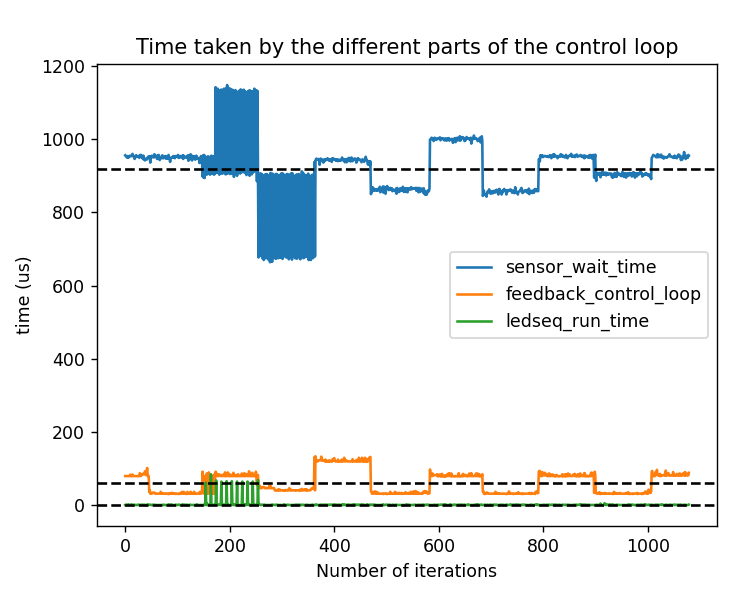
\includegraphics[width=\textwidth]{usec_reading1.png}
            \label{figure:usec_reading1}
        \end{subfigure}
        \begin{subfigure}[b]{0.48\textwidth}
            \centering
            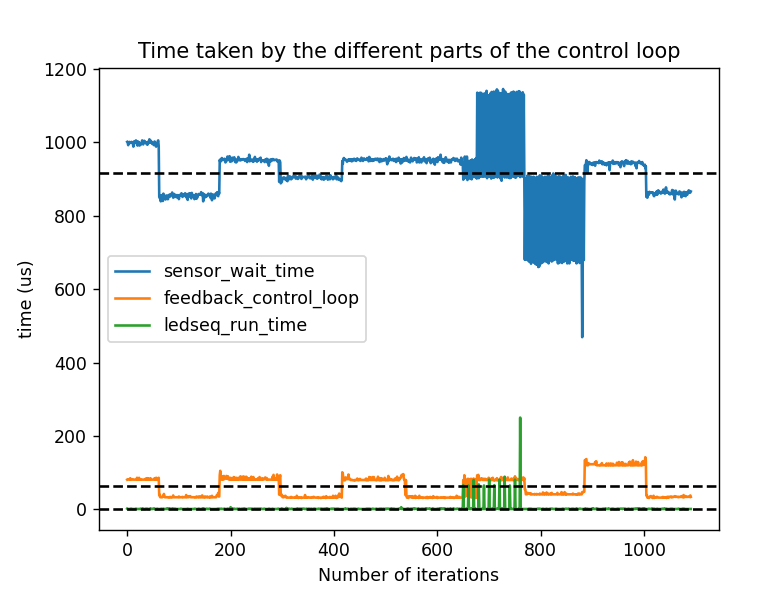
\includegraphics[width=\textwidth]{usec_reading2.png}
            \label{figure:usec_reading2}
        \end{subfigure}
        \caption{Execution time for control loop sections of Crazyflie in the non-flying state.}
        \label{figure:usec_readings1}
    \end{figure}

    \begin{figure}[hbt!]
        \centering
        \begin{subfigure}[b]{0.48\textwidth}
            \centering
            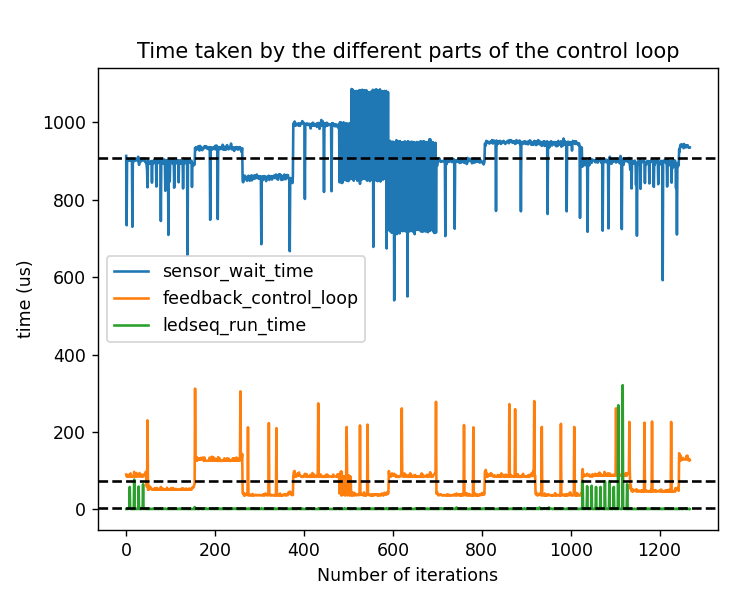
\includegraphics[width=\textwidth]{usec_reading3.png}
            \label{figure:usec_reading3}
        \end{subfigure}
        \begin{subfigure}[b]{0.48\textwidth}
            \centering
            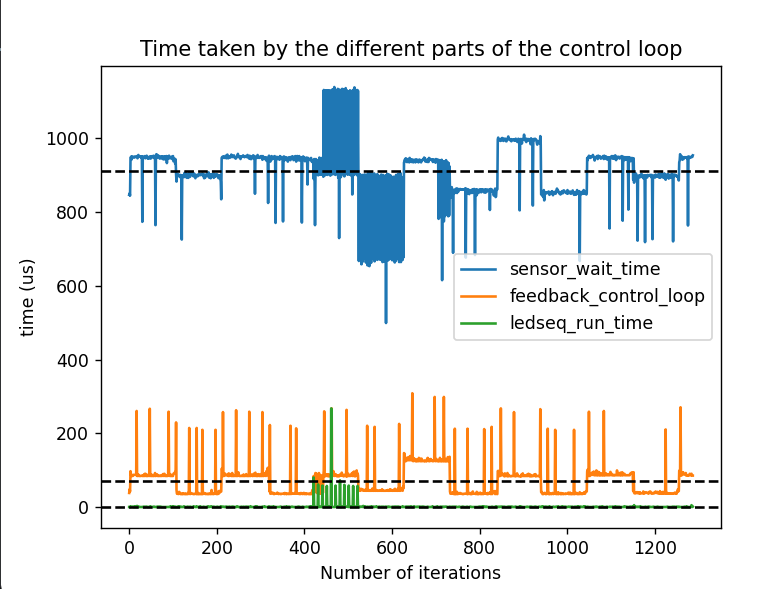
\includegraphics[width=\textwidth]{usec_reading4.png}
            \label{figure:usec_reading4}
        \end{subfigure}
        \caption{Execution time for control loop sections of Crazyflie with Extended Kalman Filter and PID controller.}
        \label{figure:usec_readings2}
    \end{figure}

    From the graphs, it is clear that the modified stabilizerTask integrated with \textFunc{ledseq\_task} is well within the $1ms$ upper bound for the feedback control loop run-time. Therefore, the timing aspect of the quadcopter is well-respected. An interesting observation, though, is that the average run-time of the three sections of stabilizerTask adds up to $1ms$. This reinforces the semantics of the code which expects the stabilzerTask to run for $1ms$. Furthermore, the relatively rough lines in figure \ref{figure:usec_readings2} compared to those in figure \ref{figure:usec_readings1} show how the feedback control loop takes longer to execute when it is in a flying state compared to when it is in a non-flying state.

    \subsection{Extended Kalman Filter}
    After successfully implementing one FreeRTOS task (\code{ledseqCmdTask}) in Heptagon, we decided to implement a second one---\code{kalmanTask}. The implementation of the Extended Kalman Filter (in the \code{kalmanTask}) is much more sophisticated than that of the Complementary Filter. It not only accepts more sensor data but also estimates the current position and velocity of the quadcopter, unlike the complementary estimator which only does that for the z-axis component (thrust) of both variables.

    \subsubsection{Reorganisation and Heptagon implementation}
    The Extended Kalman Filter or EKF is initialized in the \textFunc{estimator\_kalman.c} file in the original firmware. It is initialized as a FreeRTOS task during the system initialization and has a priority of three (appendix \ref{appendix:FreeRTOS-tasks}). In the task, the EKF algorithm proceeds as follows:
    \begin{enumerate}
        \itemsep 0em
        \item predicts the current state of the quadcopter at a frequency of $100Hz$ (appendix \ref{software-reference:EKF-predict-rate})
        \item adds the standard deviation of the process noise in every iteration of the task
        \item collects the latest measurement data from the sensors 
        \item uses the measurements to update and finalize the state estimates of the quadcopter
        \item transforms the data type of the state estimates to that accepted by the controller
    \end{enumerate}
    Out of these steps, only the sensors data collection step ($3$) interacts at the hardware level of the quadcopter. It invokes several FreeRTOS API calls, and is hence, hard to implement in Heptagon. So, with this code structure, the EKF algorithm would have to be implemented in two separate Heptagon nodes, one before the sensors call and one after that, which is undesirable. Therefore, the implementation for the EKF algorithm was reorganized  and the sensors data collection step was shifted to the very beginning of the algorithm from the middle. This code reorganization did not have any visible effects on the quadcopter during flight tests. Graphs in figure \ref{figure:usec_readings2} are in fact readings from the quadcopter running with the reorganized EKF algorithm. Essentially, this reorganisation allows the possibility of calling one Heptagon node instead of two to replace the main EKF algorithm implementation. This is not only simpler to implement but also gives clear synchronous semantics (similar to the argument in section \ref{section:controller-estimator-merging}).

    Consequently, the EKF algorithm was written in Heptagon in the \textFunc{kalman\_task} node. This node calls four nodes---\textFunc{predict\_state\_forward}, \textFunc{kalman\_core\_add\_process\_noise}, \textFunc{kalman\_core\_finalize}, and \textFunc{kalman\_core\_externalize\_state}. The first three nodes predict the current state of the quadcopter, add the standard deviation of the process noise to the predicted state, and finally update the predicted state using the current measurements from the sensors respectively. All these nodes perform their calculations using a variable of the type \textFunc{kalman\_coredata\_t} which is custom-defined in the Heptagon code. Hence, to output the final estimated state data of the quadcopter, the \textFunc{kalman\_task} node calls the \textFunc{kalman\_core\_externalize\_state} node that performs the necessary type conversions.
    
    The Heptagon code for the EKF algorithm calls several external functions like \textFunc{arm\_sqrt}, \textFunc{arm\_cos\_f32}, and \textFunc{arm\_sin\_f32} which are specific to the arm libraries and must be used to ensure fast calculations. These functions accept matrices in their original implementation, but in Heptagon, these matrices were defined as records (similar to \code{structs} in C) to maintain a clear high-level specification of the code. These custom-defined records are not recognized as intrinsic data types by the Heptagon compiler, and hence, they could not be used to communicate with external C code from inside the Heptagon code. Therefore, these records were defined in the \code{.epi} extension file instead of the Heptagon code. With this, the Heptagon code treated the record types as external data types while also allowing them to communicate with the external C code freely. For our use case, we defined the matrix type \code{covariance\_matrix} in the \code{Mathext.epi} file and it was recognized in the Heptagon code as the \code{Mathext.covariance\_matrix} type. The possibility of defining data types in the \code{.epi} extension file is a very technical detail that is not specified in the Heptagon documentation. Hence, it is described here as it is not only necessary to be utilized for the EKF algorithm but can potentially be used for other programs in the future.

    \subsubsection{Stack allocation}
    After the EKF algorithm was implemented as a Heptagon node, it was integrated into the original firmware to run parallely with the feedback control loop in the \textFunc{stabilizerTask}. Thanks to the previous reorganisation, only one node was required to be integrated which was the \textFunc{kalman\_task}. The integrated code was then tested for its correctness through flight tests. In the flight tests, it was observed through debug messages that the quadcopter was unexpectedly switching the state estimation algorithm from EKF to the Complementary Filter right after initialisation. This switching of the estimation algorithm could not be explained by looking at the code directly as the quadcopter was skipping function calls that were necessary to change the estimator type.

    The unexpected behaviour hinted at a possible stack corruption by the Heptagon-generated C code for the EKF algorithm. To confirm the hypothesis, we used the \textFunc{vApplicationStackOverflowHook()} FreeRTOS API function's second method. In FreeRTOS, a task's stack is filled with a known value when the task is first created. So, when a task is switched out of the Running state by the scheduler, this FreeRTOS function checks the last 16 bytes within the stack range. If these bytes do not correspond to the original values, the function signals that a task has been overwritten \cite{web:freertos-stack-check}. Using this API function confirmed our hypothesis as it signalled that the stack for the \textFunc{stabilizerTask} was being overwritten. To learn more about this stack overflow, we decided to use the \code{objdump} command to disassemble the object files and investigate the stack pointer. As the project was built for the arm architecture, we used the \code{arm-none-eabi-objdump} function for the disassembly. In the disassembled code, it was observed that the \textFunc{stabilzerTask} (integrated with the Heptagon code discussed until section \ref{section:ledseq-task}) needed $56$ bytes, the original C code for the EKF implementation required $60$ bytes, and the Heptagon generated C code required $476$ bytes of memory. 

    The Heptagon-generated code for EKF needed more than eight times the stack size of the task it was being integrated into and hence, the stack overflow was not surprising. The reason for the huge stack size was pinpointed to the excessive data copies performed by the Heptagon-generated C code. Normally, these data copies would be optimized and reduced by the \code{memalloc} optimization in Heptagon, but as discussed in section \ref{section:bug-in-compiler}, the optimization was found to have a bug and was hence not used. Fortunately, in the Crazyflie, FreeRTOS tasks are allocated their stacks statically. So, by modifying the stack size for the \textFunc{stabilizerTask} to nine times its original allocation, the stack overflow stopped and the quadcopter was initialized as expected. Still, during testing, the quadcopter with the Heptagon integration did not pass the initial flight tests. Due to lack of time, the Heptagon code could not be debugged and fixed any further and remains to be done in the future.

\section{Conclusion}
    The work presented in this thesis is a concrete step towards completely converting the low-level C code of the Crazyflie UAV into Heptagon. Two parts of the main feedback control loop---estimator and controller---were replicated in Heptagon whose generated C code was successfully integrated and tested in the main firmware. The thesis has also shown, by replacing the task for led sequence, how FreeRTOS tasks can be replaced with a Heptagon implementation and integrated into the main firmware.

    Some of the main results of the work are the dataflow diagrams which represent the actual code implemented in Heptagon in a synchronous manner. These diagrams make the program visually easy and simple to understand for any engineer. While implementing the original firmware in Heptagon, it was found that several variables in the data structures being passed in the functions remained unused and hence made the code needlessly complex. By streamlining the data, making it specific to each node, and clearly specifying the inputs and outputs of every node, the resulting Heptagon program was a simpler implementation of the original code. Therefore, the dataflow diagrams also reflect a more efficient interaction of the different variables and expressions in the program as they avoid any redundancy or unused code. Overall, the Heptagon adaption makes the code much more simple to understand than the same implementation in the original firmware in C. This is a very crucial aspect for complex programs that are built for UAVs where development teams regularly change. Using synchronous dataflow languages can keep the programs organized and also help in debugging because only the high-level logic needs to be correct while the implementation details are handled by the compiler. These diagrams can also potentially avoid misunderstandings between team members as they are defined by mathematical equations and relations.

    Even with the benefits of Heptagon, it still has limitations. One of the biggest strengths of C is pointers which make a program extremely fast and efficient. The Heptagon compiler, on the other hand, does not use pointers when generating the C code. This not only makes the program slow but also increases the space requirements as each new copy is allocated at a new address. A real example was observed in the implementation of the Kalman Filter where the stack size required for the Heptagon adaption was eight times larger than the original code because of the excessive data copies (they would have been less with the \code{memalloc} optimization). Furthermore, the memory allocation and management possibilities of C make it extremely powerful for implementing fast and efficient algorithms such as the fast inverse square root method in the Complementary Filter. These manipulations cannot be done in Heptagon and without them, programs will run much slower which is undesirable, especially in UAVs where decisions need to be made fast. As a result, these functions need to be externalized as C functions and doing so makes the Heptagon program open to side effects. In real-time systems such as UAVs, this a major challenge as it prevents the program to be written completely in a dataflow synchronous language while also being free of side effects and remains to be an open research problem.

\section{Further steps}
    The work in the thesis covered, amongst other things, the Extended Kalman Filter where a major portion of the original code was re-implemented in Heptagon. It was integrated into the firmware but was found to have bugs and could not be successfully tested due to a lack of time. Future debugging analysis can highlight the issues in the Heptagon implementation which should be extended to include the \code{kalmanCore} functions in the \code{src/modules/src/kalman\_core} sub-directory. \textFunc{kalman\_task} currently runs as an individual task in the original firmware, but after its integration in the \textFunc{stabilizer\_task}, it will slow the task down. Thus, it is important to study the timing aspects of the \textFunc{stabilizer\_task} (as shown in the thesis) after the Kalman integration. If needed, the frequency of the \textFunc{stabilizer\_task} can be reduced from the current $1000Hz$ to $500Hz$ as was done in Crazyflie's version $2022.05$ (appendix \ref{software-reference:stabilizer-freq}). It is important to integrate the Kalman Filter in the firmware code because it stabilizes the quadcopter far better than the Complementary Filter which cannot be used in flight tests. Moreover, if flight tests are done with the Heptagon implementation of the EKF, it presents a stronger case for Heptagon by exploiting its synchronous nature to run the UAV and at the same time providing simple and clear semantics of the program being run.

    Afterwards, the commander and other FreeRTOS tasks (appendix \ref{appendix:FreeRTOS-tasks}) should be gradually implemented in Heptagon and integrated with the original firmware. The commander has a complex implementation and uses several FreeRTOS API functions unlike the estimator and controller, and thus, will be challenging to implement in Heptagon. Eventually, by removing FreeRTOS from the firmware and running the software-specific components of the UAV solely in Heptagon, the feasibility of using a synchronous dataflow language to develop software for UAVs can be demonstrated. Furthermore, the semantics derived from that implementation can be compared with the original implementation using dataflow diagrams. This can be used to argue if the Heptagon implementation provides clearer semantics and a simple-to-understand mathematical model for the UAV compared to one that might be generated directly from the low-level C code.

\newpage
\bibliographystyle{plain}
\bibliography{main}

\newpage
% \appendix
\begin{appendices}

\section{Crazyflie feedback control loop block-diagram}
\label{appendix:previous-block-diagram}
    \begin{figure}[hbt!]
        \centering
        \begin{subfigure}[b]{0.94\textwidth}
            \centering
            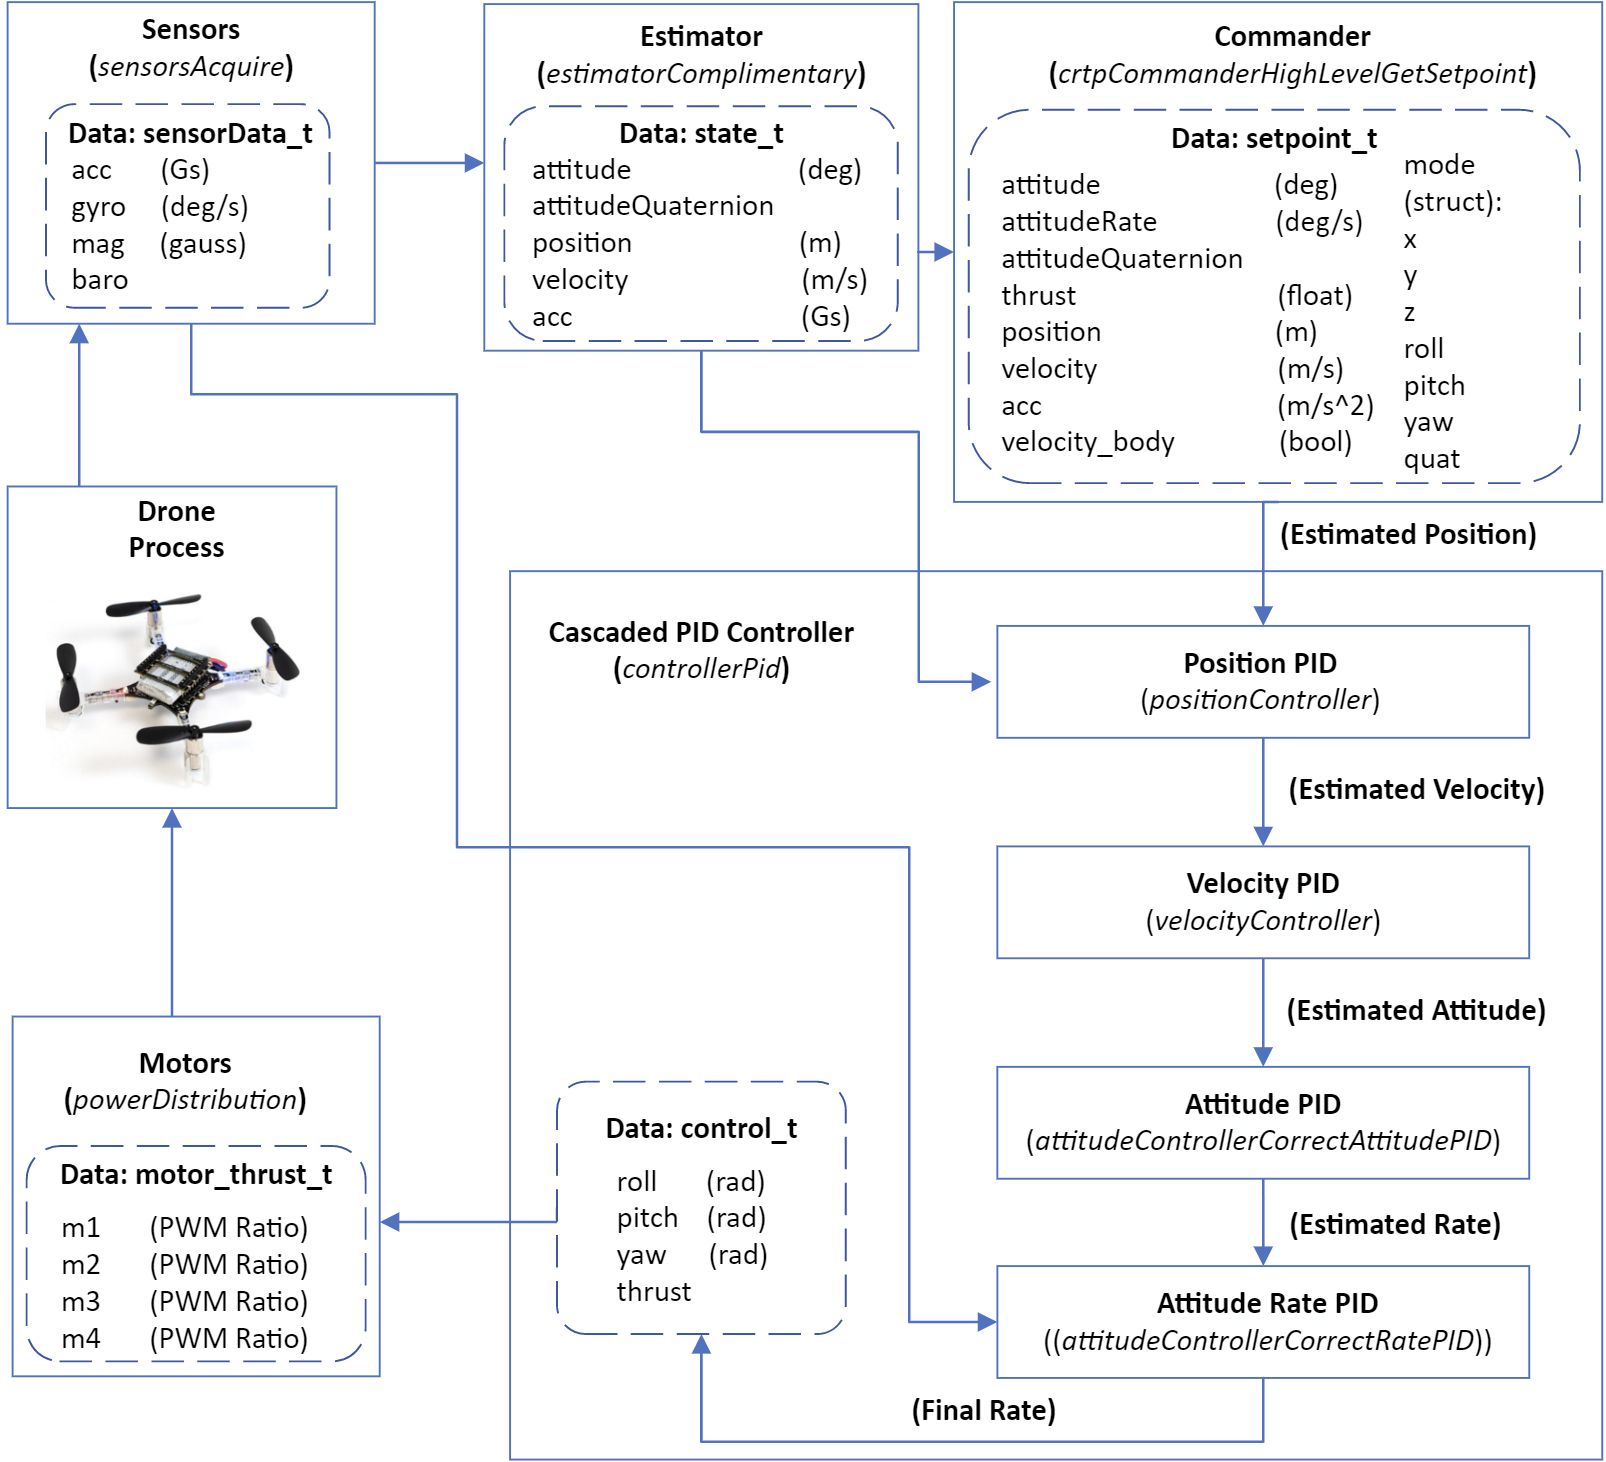
\includegraphics[width=\textwidth]{main_block.png}    
        \end{subfigure}
        \caption{Initial block-diagram for Crazyflie 2.1 control loop \cite{report:cse303-report}.}
        \label{figure:previous-block-diagram}
    \end{figure}

\section{Source code references}
\label{appendix:source-code-references}
    \def\arraystretch{1.5}
    \begin{tabular}{ N p{0.20\linewidth} | p{0.72\linewidth}}
        \hline
        \multicolumn{1}{c}{} & Definition & Url \\
        \hline
        \label{software-reference:crazyflie-github-scheduler-type} & FreeRTOS scheduler type & \url{https://github.com/bitcraze/crazyflie-firmware/blob/79aead2deafe0f9c5134422566c2f80e2db96613/src/config/FreeRTOSConfig.h#L73} \\
        \label{software-reference:crazyflie-github-maxTaskPriority} & maxTaskPriority & \url{https://github.com/bitcraze/crazyflie-firmware/blob/79aead2deafe0f9c5134422566c2f80e2db96613/src/config/FreeRTOSConfig.h#L93} \\
        \label{software-reference:crazyflie-max-log-len} & maxLogLen & \url{https://github.com/bitcraze/crazyflie-lib-python/blob/master/cflib/crazyflie/log.py#L135} \\
        \label{software-reference:stabilizer-task-priority} & stabilizerTask Priority & \url{https://github.com/bitcraze/crazyflie-firmware/blob/b84db29c5311ff44a833ce05639b03768a9201f3/src/config/config.h#L67} \\
        \label{software-reference:stabilizer-freq} & stabilizer frequency & \url{https://github.com/bitcraze/crazyflie-firmware/blob/8e63e810b0778bc958b3473c5f8043a6fce9d122/src/modules/src/stabilizer.c#L214} \\
        \label{software-reference:commander-freq} & commander frequency & \url{https://github.com/bitcraze/crazyflie-firmware/blob/aaeaf11658ca8b3891b67f187fbc941d6aadd7bc/src/modules/interface/stabilizer_types.h#L367} \\
        \label{software-reference:tick-rate} & FreeRTOS Tick Rate & \url{https://github.com/bitcraze/crazyflie-firmware/blob/79aead2deafe0f9c5134422566c2f80e2db96613/src/config/FreeRTOSConfig.h#L77} \\
        \label{software-reference:invSqrt} & fast inverse square root & \url{https://github.com/id-Software/Quake-III-Arena/blob/master/code/game/q_math.c#L552} \\
        \label{software-reference:EKF-predict-rate} & EKF prediction rate & \url{https://github.com/bitcraze/crazyflie-firmware/blob/9371e5f5036e8619374db403f9e3141a2e10aa7c/src/modules/src/estimator/estimator_kalman.c#L115} \\
        \hline
    \end{tabular}


\section{FreeRTOS tasks used in Crazyflie 2.1}
\label{appendix:FreeRTOS-tasks}
    \def\arraystretch{1.5}
    \begin{tabular}{ |l|c|l|c| }
        \hline
        Task Name & Task Priority & Task Name & Task Priority\\
        \hline
        stabilizerTask & 5 & logTask & 1 \\
        sesnorsTask & 4 & ParamTask & 1 \\
        sysLinkTask & 3 & memTask & 1 \\ 
        CRTPCommanderhighLevelTask & 2 & pmTask & 0 \\
        kalmanTask & 2 & CRTPServiceTask & 0 \\
        systemTask & 2 & platformServiceTask & 0 \\
        ledseqCmdTask & 1 & & \\
        \hline
    \end{tabular}

\clearpage
\section{node estimator\_complementary}
    \label{appendix:estimator-node}
        \bigskip
    \begin{lstlisting}[language=C]
node estimator_complementary(sensor: sensor_data_est)
returns (st : state_t);
var freq_att_update, freq_pos_update : bool;
    last grav: vec3 = {x = 0.0; y = 0.0; z = 0.0};
    last st_attitude_this: attitude = {roll = 0.0; pitch = 0.0; yaw = 0.0};
    last st_attitude_quat_this: quaternion = {qw = 1.0; qx = 0.0; qy = 0.0; qz = 0.0};
    last st_acc_z: float = 0.0;
    last baseZacc: float = 0.0;
    last velocityZ: float = 0.0;
    last st_position_z: float = 0.0;
    last st_velocity_z: float = 0.0;
let
    freq_att_update = everyn<<4>>();
    freq_pos_update = everyn<<10>>();

    switch freq_att_update
    | true do
        (st_attitude_quat_this, grav, baseZacc) = sensfusion6_update_Q(sensor.gyro_est, sensor.acc_est);
        st_attitude_this = sensfusion6_get_euler_rpy(st_attitude_quat_this, grav);
        st_acc_z =  (  (sensor.acc_est.x *. grav.x) 
                    +. (sensor.acc_est.y *. grav.y) 
                    +. (sensor.acc_est.z *. grav.z)
                    ) -. baseZacc;
        velocityZ = position_update_velocity(st_acc_z, last velocityZ);
    | false do
    end;

    switch freq_pos_update
    | true do
        (st_position_z, st_velocity_z) = 
            positionEstimate(sensor.baro_est, sensor.tof, velocityZ);
    | false do
    end;

    st = {  st_attitude = st_attitude_this;
            st_attitude_quat = st_attitude_quat_this;
            st_position = {x = 0.0; y = 0.0; z = st_position_z};
            st_velocity = {x = 0.0; y = 0.0; z = st_velocity_z};
            st_acc = {x = 0.0; y = 0.0; z = st_acc_z}}; |\label{line:acc_bug}|
tel
\end{lstlisting}
    \bigskip

\end{appendices}

\end{document}